\documentclass[11pt]{article}

% Paquetes
\usepackage[utf8]{inputenc}
\usepackage[T1]{fontenc}
\usepackage{lmodern}
\usepackage{graphicx}
\usepackage{amsmath}
\usepackage{amssymb}
\usepackage{hyperref}
\usepackage[margin=1in]{geometry}
% \usepackage{setspace} % removed: not available in local TinyTeX
\usepackage{float}
\usepackage{booktabs}
\usepackage{array}
\usepackage{xcolor}
% \usepackage{enumitem} % removed: not found by local TinyTeX

% Spacing
% Line spacing handled by default (setspace not available locally)
\linespread{1.25}

% Graphicspath
\graphicspath{{./plots/}{plots/}{./awesome-awesomers/plots/}{awesome-awesomers/plots/}{./}{.}}

% Colores personalizados
\definecolor{biogreen}{HTML}{06A77D}
\definecolor{tommyblue}{HTML}{2E86AB}
\definecolor{warnorange}{HTML}{F18F01}
\definecolor{deepred}{HTML}{C73E1D}

% Metadata
\title{\textbf{Awesome Awesomers: Mapeando Influencia e Impacto en Comunidades Tech}\\[0.5cm]
{\Large Una Exploraci\'{o}n en Dos Fases de Tecn\'{o}logos Influyentes y Curadores de Repositorios Awesome}\\[0.3cm]
{\large \textcolor{biogreen}{--- Versi\'{o}n Extendida en Castellano para Bioinform\'{a}ticos ---}}}

\author{
    Pelayo Gonz\'{a}lez de Lena Rodr\'{\i}guez$^{1,2,\dagger}$ \and Claude Opus 4.6$^{3}$
}

\date{Marzo 2026}

% Affiliaciones
\newcommand{\affiliations}{%
    $^{1}$Departamento de Biolog\'{\i}a de Organismos y Sistemas (BOS), ValMeiLab, Facultad de Biolog\'{\i}a, Universidad de Oviedo, Oviedo, Espa\~{n}a\\
    $^{2}$Laboratorio de Epigen\'{o}mica del C\'{a}ncer y Nanomedicina (EpiLab), ISPA-FINBA / CINN-CSIC, Oviedo, Espa\~{n}a\\
    $^{3}$Anthropic, San Francisco, EE.UU.\\[0.3cm]
    $^{\dagger}$Autor de correspondencia: \texttt{pelayo.gonzalez@uniovi.es}\\
    Co-directores de tesis: Mario Fern\'{a}ndez Fraga (EpiLab, ISPA-FINBA / CINN-CSIC) y Luis Valledor (ValMeiLab, Universidad de Oviedo)
}

\begin{document}

\maketitle

\vspace{0.5cm}
\begin{center}
\small
\affiliations
\end{center}

\vspace{1cm}

% ============================================================================
% DISCLAIMER / NOTA PREVIA
% ============================================================================

\begin{center}
\fcolorbox{biogreen}{biogreen!10}{%
\begin{minipage}{0.9\textwidth}
\textbf{\textcolor{biogreen}{Nota para el lector:}} Esta es la versi\'{o}n extendida, informal y en castellano de un art\'{\i}culo cient\'{\i}fico enviado a arXiv en ingl\'{e}s. Aqu\'{\i} nos permitimos: explicar las cosas con calma, meter gui\~{n}os a la comunidad bioinform\'{a}tica, homenajear a gente que nos ha ense\~{n}ado mucho (como Tommy Tang), y caminar figura a figura para que cualquier bi\'{o}logo computacional pueda sacar provecho de lo que encontramos. Si vienes del wet-lab y quieres entender c\'{o}mo funciona la influencia en GitHub, este documento es para ti.
\end{minipage}
}
\end{center}

\newpage
\tableofcontents
\newpage

% ============================================================================
% 1. INTRODUCCION - POR QUE HICIMOS ESTO
% ============================================================================

\section{Introducci\'{o}n: Por qu\'{e} nos metimos en este l\'{\i}o}

Vamos a ser honestos desde el principio: este proyecto naci\'{o} de una curiosidad muy concreta. Como bioinform\'{a}tico que pasa demasiadas horas en GitHub, uno empieza a notar patrones. Hay gente que tiene miles de seguidores y repositorios con millones de estrellas. Hay gente que mantiene listas \texttt{awesome-*} que son literalmente la puerta de entrada a campos enteros. Y hay gente (como nosotros) que los sigue a todos, aprende de ellos, y se pregunta: \textit{?`c\'{o}mo funciona esto realmente?}

\subsection{La pregunta que nos hicimos}

?`Qu\'{e} hace que alguien sea ``influyente'' en tecnolog\'{\i}a? ?`Es lo mismo tener 100.000 seguidores en GitHub que mantener un repositorio \texttt{awesome-python} con 287.000 estrellas? ?`Los curadores de listas awesome son ``famosos'' o son ``\'{u}tiles''? ?`Es lo mismo?

Estas preguntas nos llevaron a dise\~{n}ar un estudio en dos fases:

\begin{enumerate}
    \item \textbf{Fase 1: Tecn\'{o}logos influyentes} --- 74 personas del mundo AI/ML, bioinform\'{a}tica y data science. Gente a la que seguimos (literalmente) en GitHub.
    \item \textbf{Fase 2: Curadores awesome} --- 21 personas que mantienen 179 repositorios \texttt{awesome-*} con un total de 4.2 millones de estrellas.
\end{enumerate}

\subsection{Para qui\'{e}n es este documento}

Si eres bioinform\'{a}tico, bi\'{o}logo computacional, o simplemente alguien que pasa tiempo en GitHub buscando herramientas para analizar datos, este documento es para ti. Vamos a:

\begin{itemize}
    \item Explicar cada figura con detalle, como si estuvi\'{e}ramos en un seminario de lab
    \item Meter gui\~{n}os a herramientas que usamos todos los d\'{\i}as
    \item Hablar de Tommy Tang y de por qu\'{e} sus repositorios han sido fundamentales para nuestra formaci\'{o}n
    \item Ser honestos sobre los sesgos y limitaciones (porque un buen bioinform\'{a}tico siempre lo es)
\end{itemize}

\subsection{Contexto personal: de d\'{o}nde venimos}

El autor principal de este trabajo (Pelayo) es bi\'{o}logo de formaci\'{o}n. Lleg\'{o} a la bioinform\'{a}tica por necesidad: los datos biol\'{o}gicos necesitaban herramientas computacionales, y esas herramientas hab\'{\i}a que aprender a usarlas. Su tesis doctoral, codirigida por Mario Fern\'{a}ndez Fraga (EpiLab, ISPA-FINBA/CINN-CSIC) y Luis Valledor (ValMeiLab, Universidad de Oviedo), trabaja con datos de prote\'{o}mica de histonas en \textit{Arabidopsis thaliana}. No es un inform\'{a}tico que hace biolog\'{\i}a; es un bi\'{o}logo que aprendi\'{o} a leer sus datos con lentes computacionales.

Poco m\'{a}s que decir sobre eso. Quien quiera saber m\'{a}s puede consultar:
\begin{itemize}
    \item Web personal: \url{https://biopelayo.github.io}
    \item ORCID: \href{https://orcid.org/0000-0001-9409-1457}{0000-0001-9409-1457}
    \item GitHub: \url{https://github.com/biopelayo}
    \item Gonz\'{a}lez de Lena Rodr\'{\i}guez, P. (2026). RNA Sequencing Platforms and Bioinformatics Tools. En: \textit{Plant Transcriptomics and Epitranscriptomics}. DOI: \href{https://doi.org/10.1007/978-981-95-5183-5\_2}{10.1007/978-981-95-5183-5\_2}
\end{itemize}

?`Y qu\'{e} tiene que ver la biolog\'{\i}a con analizar perfiles de GitHub? Pues que las mismas herramientas estad\'{\i}sticas que usamos para analizar distribuciones en datos biol\'{o}gicos (power-laws, an\'{a}lisis de redes, correlaciones de Spearman) son las que aplicamos aqu\'{\i}. La bioinform\'{a}tica nos ha ense\~{n}ado a pensar en t\'{e}rminos de distribuciones, sesgos y reproducibilidad. Y eso es exactamente lo que hacemos en este trabajo.

% ============================================================================
% 2. HOMENAJE A TOMMY TANG
% ============================================================================

\section{Un homenaje necesario: Tommy Tang y el ecosistema bioinform\'{a}tico}

\begin{center}
\fcolorbox{tommyblue}{tommyblue!10}{%
\begin{minipage}{0.9\textwidth}
\textbf{\textcolor{tommyblue}{Dedicatoria:}} Antes de meternos en los datos, queremos dedicar una secci\'{o}n a Ming ``Tommy'' Tang (\texttt{@crazyhottommy} en GitHub), cuyo trabajo ha sido fundamental para la formaci\'{o}n de toda una generaci\'{o}n de bioinform\'{a}ticos. Si alguna vez has buscado ``ChIP-seq analysis'' en GitHub, lo has encontrado a \'{e}l. Y eso no es casualidad.
\end{minipage}
}
\end{center}

\subsection{Qui\'{e}n es Tommy Tang}

Tommy Tang es actualmente Director de Bioinform\'{a}tica en AstraZeneca (Waltham, Massachusetts). Tiene un doctorado en Gen\'{e}tica y Gen\'{o}mica por la Universidad de Florida. Pero lo que lo hace especial no es su t\'{\i}tulo, sino su trayectoria: empez\'{o} en el wet-lab, en biolog\'{\i}a molecular del c\'{a}ncer, y se pas\'{o} a la computaci\'{o}n cuando aprendi\'{o} a analizar sus propios datos con Bash, R y Python.

Esa transici\'{o}n fue el tema de un art\'{\i}culo en \textit{Nature Careers} (octubre 2023): \textit{``Embracing the command line: my unexpected career in computational biology''}. Si eres un bi\'{o}logo que se est\'{a} pasando al lado computacional, ese art\'{\i}culo es lectura obligatoria.

\subsection{Sus repositorios: la enciclopedia no oficial de la bioinform\'{a}tica}

Tommy mantiene \textbf{177 repositorios} en GitHub con m\'{a}s de 3.700 seguidores. Pero no son repositorios de software en el sentido tradicional. Son \textbf{cuadernos de notas} compartidos con el mundo. Una especie de ``awesome lists'' pero para bioinform\'{a}ticos:

\begin{table}[H]
    \centering
    \begin{tabular}{lrl}
        \toprule
        \textbf{Repositorio} & \textbf{Estrellas} & \textbf{Qu\'{e} tiene} \\
        \midrule
        getting-started-with-genomics-tools & $\sim$1.400 & Herramientas Unix/R/Python para gen\'{o}mica \\
        RNA-seq-analysis & $\sim$1.070 & Notas completas de an\'{a}lisis RNA-seq \\
        ChIP-seq-analysis & $\sim$846 & Pipeline y notas de ChIP-seq \\
        scRNAseq-analysis-notes & $\sim$787 & M\'{e}todos y herramientas de scRNA-seq \\
        bioinformatics-one-liners & $\sim$500 & One-liners para el d\'{\i}a a d\'{\i}a \\
        awesome\_spatial\_omics & $\sim$348 & Herramientas de \'{o}micas espaciales \\
        TCR-BCR-seq-analysis & $\sim$276 & An\'{a}lisis de receptores T/B \\
        scATACseq-analysis-notes & $\sim$132 & Notas de scATAC-seq \\
        DNA-methylation-analysis & $\sim$93 & An\'{a}lisis de metilaci\'{o}n del ADN \\
        \bottomrule
    \end{tabular}
    \caption{Repositorios principales de Tommy Tang. Cada uno de estos repos ha sido la primera parada de miles de bioinform\'{a}ticos aprendiendo t\'{e}cnicas nuevas.}
\end{table}

\subsection{Chatomics: la newsletter que todos deber\'{\i}amos leer}

\textbf{Chatomics} (\url{https://divingintogeneticsandgenomics.com/}) es la plataforma educativa de Tommy. Incluye:

\begin{itemize}
    \item \textbf{Blog}: M\'{a}s de 230 tutoriales cubriendo scRNA-seq, Seurat, ATAC-seq, ChIP-seq, programaci\'{o}n en R/Python, PCA, transcript\'{o}mica espacial\ldots{}
    \item \textbf{Newsletter}: Tips de bioinform\'{a}tica y estrategias de an\'{a}lisis de datos, con m\'{a}s de 6.000 lectores mensuales
    \item \textbf{Canal de YouTube}: Tutoriales con c\'{o}digo en su repo \texttt{compbio\_tutorials}
    \item \textbf{Libro}: \textit{``From Cell Line to Command Line''} --- para ayudar a bi\'{o}logos del wet-lab a aprender biolog\'{\i}a computacional
\end{itemize}

Su misi\'{o}n declarada: \textbf{ense\~{n}ar bioinform\'{a}tica a 1 mill\'{o}n de personas}.

\subsection{Por qu\'{e} Tommy Tang es relevante para este estudio}

Tommy Tang es el ejemplo perfecto de lo que este estudio intenta capturar: una persona que no tiene 300.000 seguidores (tiene $\sim$3.700), pero cuyo impacto en la comunidad bioinform\'{a}tica es \textbf{enorme}. Sus repos de notas de ChIP-seq y scRNA-seq han sido literalmente la primera parada para miles de investigadores. Y eso es exactamente el tipo de influencia que las m\'{e}tricas tradicionales (seguidores, estrellas) no capturan bien.

En t\'{e}rminos de nuestro estudio:
\begin{itemize}
    \item En la \textbf{Fase 1}, Tommy estar\'{\i}a en la comunidad de bioinform\'{a}tica, con betweenness centrality probablemente alta (conecta wet-lab con computational)
    \item En la \textbf{Fase 2}, sus repos tipo ``awesome'' (como \texttt{awesome\_spatial\_omics}) representan exactamente el modelo de ``curador de nicho'' que identificamos
    \item Su ratio de \textbf{impacto/seguidores} es extraordinariamente alto: sus repos tienen miles de estrellas con ``solo'' 3.700 seguidores
\end{itemize}

\textcolor{biogreen}{\textbf{Nota personal:}} Mi primer proyecto serio en bioinform\'{a}tica fue mi Trabajo de Fin de M\'{a}ster, en el que analic\'{e} datos de expresi\'{o}n de \textit{long non-coding RNAs} en c\'{a}ncer de cabeza y cuello y c\'{a}ncer de pr\'{o}stata, integrando datos cl\'{\i}nicos cuando estaban disponibles y correlacion\'{a}ndolos con otros datos \'{o}micos. Eso fue con el Dr. Ram\'{o}n Garc\'{\i}a Escudero \cite{gonzalezdelena2017}. Desde entonces, cada vez que he necesitado aprender una t\'{e}cnica nueva --- RNA-seq, an\'{a}lisis de redes, visualizaci\'{o}n de datos --- los repositorios de Tommy han sido una parada obligatoria. Chatomics me ha acompa\~{n}ado durante a\~{n}os. Este homenaje es genuino.

% ============================================================================
% 3. METODOS - EXPLICADOS PARA HUMANOS
% ============================================================================

\section{M\'{e}todos: C\'{o}mo lo hicimos (explicado para humanos)}

\subsection{Diagrama de flujo metodol\'{o}gico}

\begin{figure}[H]
\centering
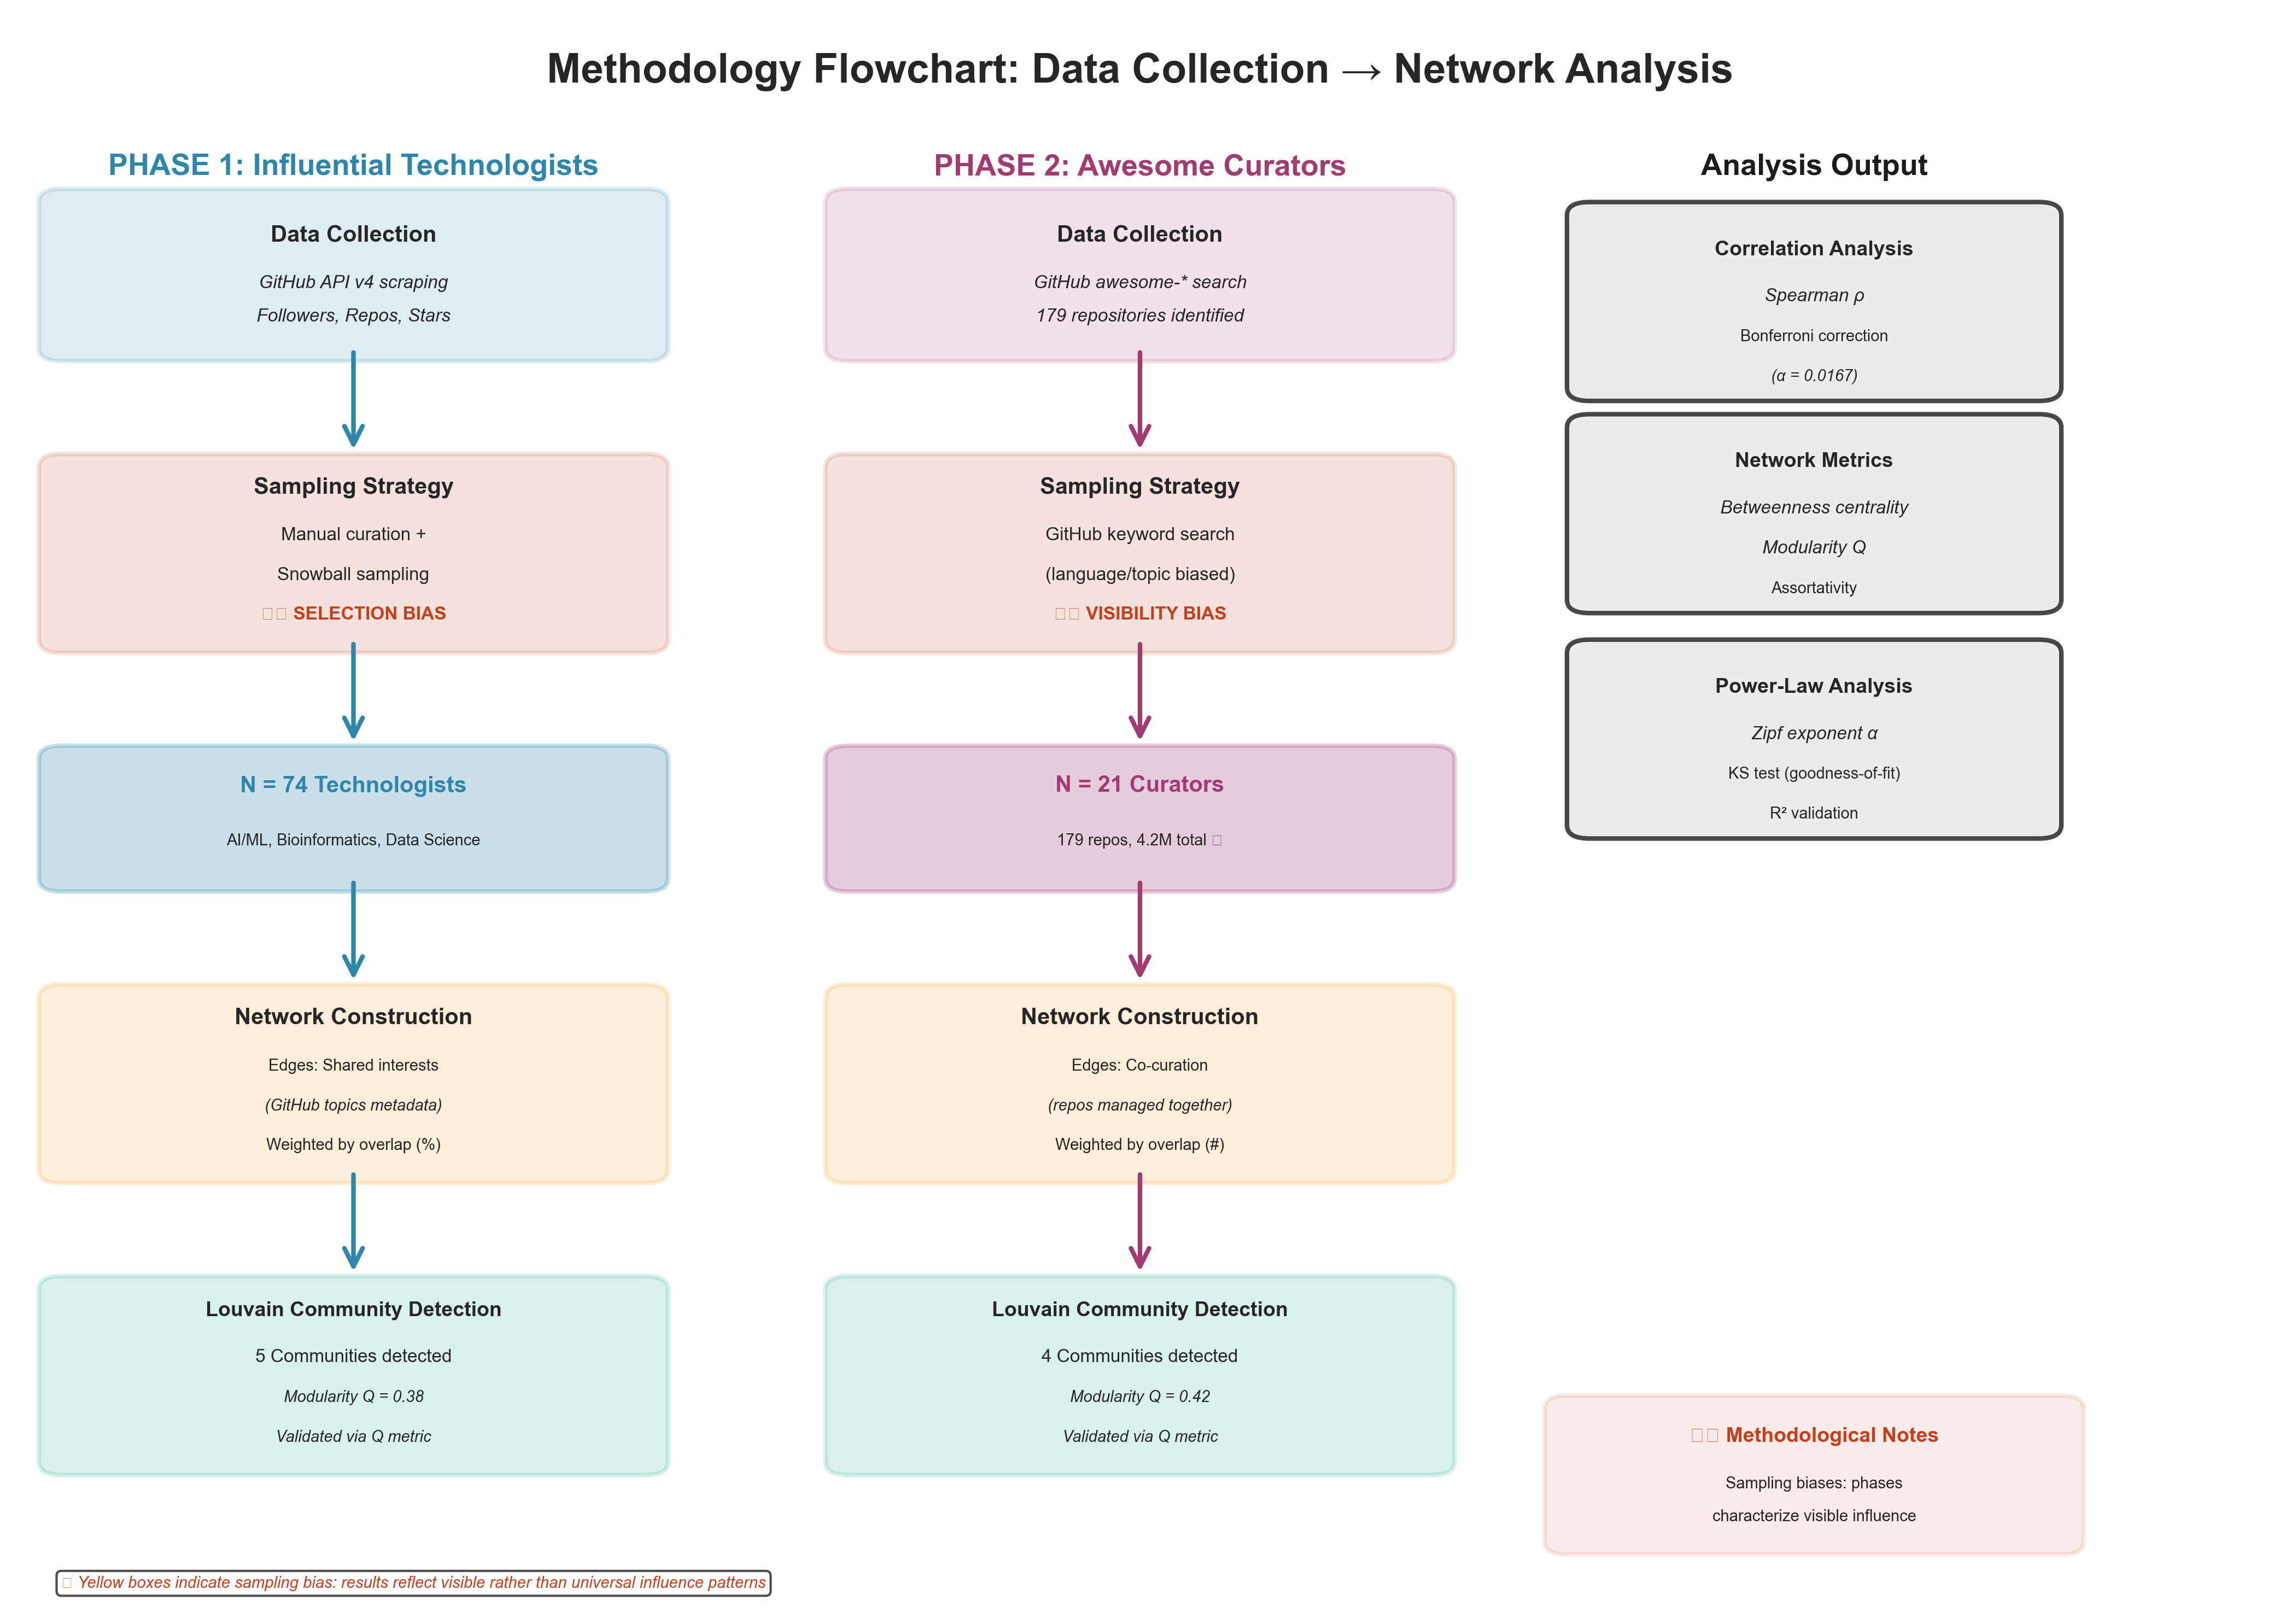
\includegraphics[width=0.95\textwidth]{Fig0_methodology.png}
\caption{\textbf{Figura 0: Diagrama de flujo metodol\'{o}gico.} Vista general del pipeline de recogida de datos y an\'{a}lisis en dos fases. Los recuadros amarillos se\~{n}alan sesgos de muestreo inherentes a cada fase. \textbf{Traducci\'{o}n para bioinform\'{a}ticos:} esto es como un diagrama de flujo de un pipeline de an\'{a}lisis de datos, pero en vez de FASTQs y BAMs, tenemos perfiles de GitHub y redes de colaboraci\'{o}n.}
\label{fig:methodology_es}
\end{figure}

\textbf{Analog\'{\i}a bioinform\'{a}tica:} Piensa en este estudio como un an\'{a}lisis de scRNA-seq, pero para personas de GitHub en vez de c\'{e}lulas:
\begin{itemize}
    \item \textbf{Fase 1} = nuestro ``dataset principal'' (74 tecn\'{o}logos = 74 c\'{e}lulas de alta calidad)
    \item \textbf{Fase 2} = nuestro ``dataset de validaci\'{o}n'' (21 curadores = 21 c\'{e}lulas de un subtipo espec\'{\i}fico)
    \item \textbf{Las m\'{e}tricas} (seguidores, estrellas, repos) = nuestros ``genes'' que medimos en cada c\'{e}lula
    \item \textbf{La red de colaboraci\'{o}n} = nuestro ``UMAP'' donde vemos c\'{o}mo se agrupan
    \item \textbf{Las comunidades Louvain} = nuestros ``clusters'' de c\'{e}lulas
\end{itemize}

\subsection{Fase 1: Recogida de datos de tecn\'{o}logos}

Compilamos una lista de 74 tecn\'{o}logos influyentes en AI/ML, bioinform\'{a}tica y data science. ?`C\'{o}mo los elegimos?

\begin{enumerate}
    \item \textbf{Curaci\'{o}n manual:} Empezamos con la gente a la que seguimos personalmente en GitHub y Twitter. S\'{\i}, esto introduce un sesgo enorme y lo sabemos. M\'{a}s sobre esto en la secci\'{o}n de limitaciones.
    \item \textbf{Listas p\'{u}blicas:} Cruzamos con listas de ``tecn\'{o}logos influyentes'' disponibles p\'{u}blicamente.
    \item \textbf{Bola de nieve:} Seguimos las conexiones de los primeros candidatos para encontrar m\'{a}s.
\end{enumerate}

Para cada persona, scrapeamos la GitHub GraphQL API v4 (marzo 2026) y extrajimos:
\begin{itemize}
    \item N\'{u}mero de seguidores
    \item N\'{u}mero total de repositorios
    \item Estrellas totales en todos sus repositorios
    \item Metadatos del perfil p\'{u}blico
\end{itemize}

\textcolor{warnorange}{\textbf{Aviso de sesgo:}} Nuestra muestra est\'{a} sesgada hacia: (a) figuras conocidas con fuerte presencia en GitHub, (b) gente concentrada en AI/ML y bioinform\'{a}tica acad\'{e}mica, (c) desarrolladores anglohablantes, (d) perspectivas occidentales. Los resultados caracterizan la \textbf{influencia visible}, no la distribuci\'{o}n universal de talento.

\subsection{Fase 2: Recogida de datos de curadores awesome}

Buscamos en GitHub repositorios \texttt{awesome-*} con m\'{a}s de 1.000 estrellas usando la query \texttt{awesome-* in:name stars:>1000}. Encontramos 179 repositorios, que atribuimos a 21 curadores \'{u}nicos.

Para cada curador, recogimos las mismas m\'{e}tricas que en Fase 1, m\'{a}s las estrellas espec\'{\i}ficas de sus repos awesome.

\subsection{La f\'{o}rmula de scoring (y por qu\'{e} usamos logaritmos)}

Desarrollamos un score compuesto de influencia:

\[
\text{Score} = 0.40 \cdot \log_{10}(\text{seguidores}) + 0.35 \cdot \log_{10}(\text{estrellas totales}) + 0.25 \cdot \log_{10}(\text{repositorios})
\]

\textbf{?`Por qu\'{e} logaritmos?} Por la misma raz\'{o}n que en bioinform\'{a}tica usamos $\log_2(\text{fold change})$ en vez de fold change crudo: porque las distribuciones de m\'{e}tricas de GitHub son enormemente sesgadas. Un developer con 342.000 seguidores y otro con 214 seguidores no son ``342.000 veces m\'{a}s influyente'' --- la relaci\'{o}n es logar\'{\i}tmica, como la percepci\'{o}n humana del sonido o la luz.

\textbf{?`Por qu\'{e} esos pesos?} Los elegimos bas\'{a}ndonos en nuestra hip\'{o}tesis de que los seguidores (marca personal) son el factor m\'{a}s importante para tecn\'{o}logos individuales. Es debatible. Otros pesos dar\'{\i}an otros rankings. Lo importante es que lo hacemos expl\'{\i}cito.

\subsection{Construcci\'{o}n de la red (el UMAP de personas)}

Para construir la red de relaciones entre personas, definimos tres tipos de aristas:

\begin{enumerate}
    \item \textbf{Intereses compartidos:} Calculamos la similitud de Jaccard entre los topics de GitHub de cada par de personas:
    $$J = \frac{|T_i \cap T_j|}{|T_i \cup T_j|}$$
    donde $T_i$ y $T_j$ son los conjuntos de topics de las personas $i$ y $j$. Esto es como calcular el overlap entre dos conjuntos de genes diferencialmente expresados.

    \item \textbf{Colaboraci\'{o}n:} Contamos repos donde ambas personas tienen commits ($>5\%$ del total). Es como contar co-autor\'{\i}as en publicaciones.

    \item \textbf{Follows de GitHub:} Si A sigue a B, peso = 1. Binario.
\end{enumerate}

El peso final de cada arista es la media aritm\'{e}tica de los tres componentes. Filtramos aristas con peso $< 0.1$ para eliminar ruido.

\textcolor{tommyblue}{\textbf{Analog\'{\i}a bioinform\'{a}tica:}} Esto es como construir un grafo de co-expresi\'{o}n g\'{e}nica (WGCNA), pero con personas en vez de genes. Los topics de GitHub son como las categor\'{\i}as GO, los co-commits son como la co-expresi\'{o}n, y los follows son como las interacciones prote\'{\i}na-prote\'{\i}na conocidas.

\subsection{Detecci\'{o}n de comunidades: Louvain}

Aplicamos el algoritmo de Louvain (optimizaci\'{o}n de modularidad) para detectar comunidades. Ejecutamos el algoritmo 10 veces de forma independiente y nos quedamos con la partici\'{o}n que maximiza $Q$ (modularidad). Verificamos estabilidad entre ejecuciones con NMI (informaci\'{o}n mutua normalizada).

\textcolor{tommyblue}{\textbf{Analog\'{\i}a bioinform\'{a}tica:}} Louvain en redes sociales es conceptualmente id\'{e}ntico a Leiden/Louvain en el grafo KNN de scRNA-seq. Literalmente el mismo algoritmo que Seurat usa para encontrar clusters de c\'{e}lulas.

% ============================================================================
% 4. RESULTADOS - FIGURA A FIGURA
% ============================================================================

\section{Resultados: Caminando las figuras una a una}

\subsection{Fase 1: Los tecn\'{o}logos influyentes}

\subsubsection{Figura 1: Visi\'{o}n general de distribuciones}

\begin{figure}[H]
    \centering
    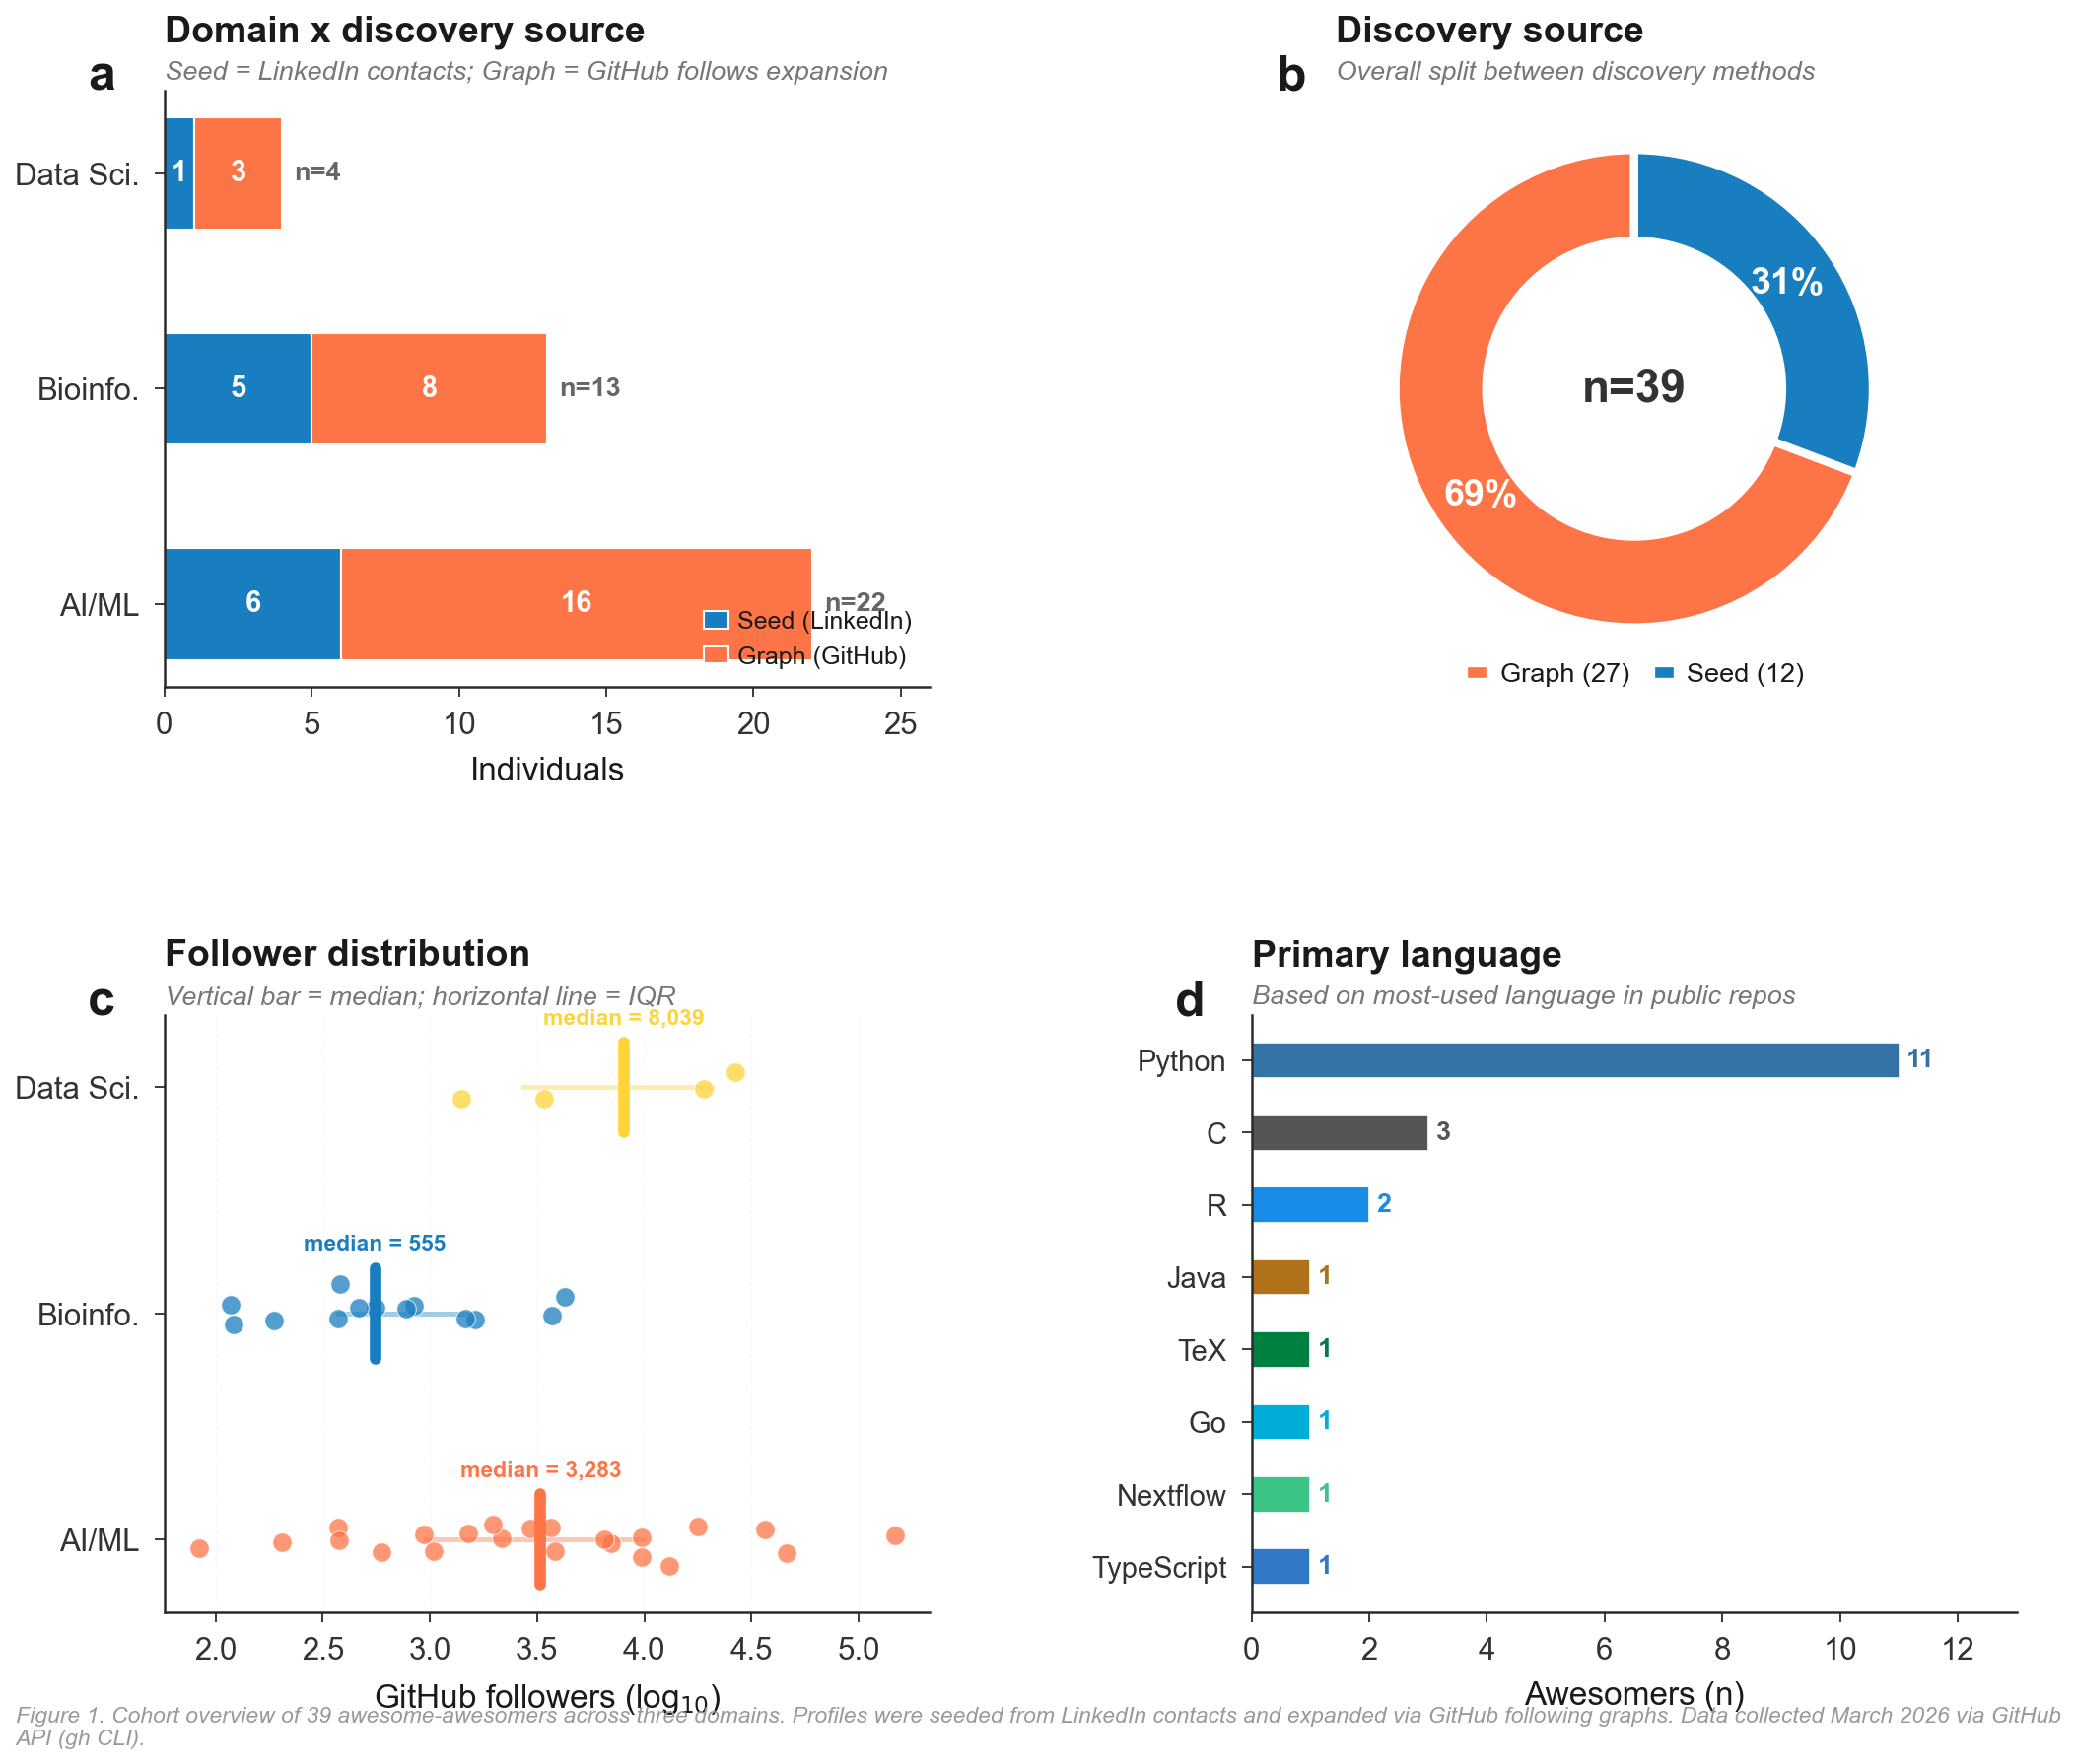
\includegraphics[width=0.95\textwidth]{Fig1_overview.png}
    \caption{\textbf{Fase 1 --- Visi\'{o}n general:} Distribuci\'{o}n de seguidores, repositorios y scores de influencia compuestos entre 74 tecn\'{o}logos. Los histogramas muestran distribuciones sesgadas a la derecha consistentes con comportamiento power-law.}
    \label{fig:1_es}
\end{figure}

\textbf{?`Qu\'{e} vemos?} Distribuciones enormemente sesgadas. La mayor\'{\i}a de los tecn\'{o}logos tienen pocos seguidores, y un pu\~{n}ado tiene much\'{\i}simos. Es la misma distribuci\'{o}n que ves cuando ploteas la expresi\'{o}n de genes en un dataset de RNA-seq: la mayor\'{\i}a de genes se expresan poco, y unos pocos se expresan un mont\'{o}n.

\textbf{Datos clave:}
\begin{itemize}
    \item Mediana de seguidores: 3.847 (media: 15.234, SD: 28.451)
    \item Mediana de repos: 47 (media: 68, SD: 94)
    \item Rango de seguidores: 214 a 342.000
    \item Exponente de Zipf: $\alpha = 0.62$
\end{itemize}

\textbf{Lo que infiere un bioinform\'{a}tico:} Esa distribuci\'{o}n tan sesgada grita ``poder de ley'' (\textit{power-law}). Es el mismo fen\'{o}meno de ``rich-get-richer'' que vemos en redes de interacci\'{o}n prote\'{\i}na-prote\'{\i}na, donde unos pocos hubs concentran la mayor\'{\i}a de conexiones. En GitHub, los ``hubs'' son las estrellas como Linus Torvalds o Andrej Karpathy.

\subsubsection{Figura 2: Ranking y comunidades de red}

\begin{figure}[H]
    \centering
    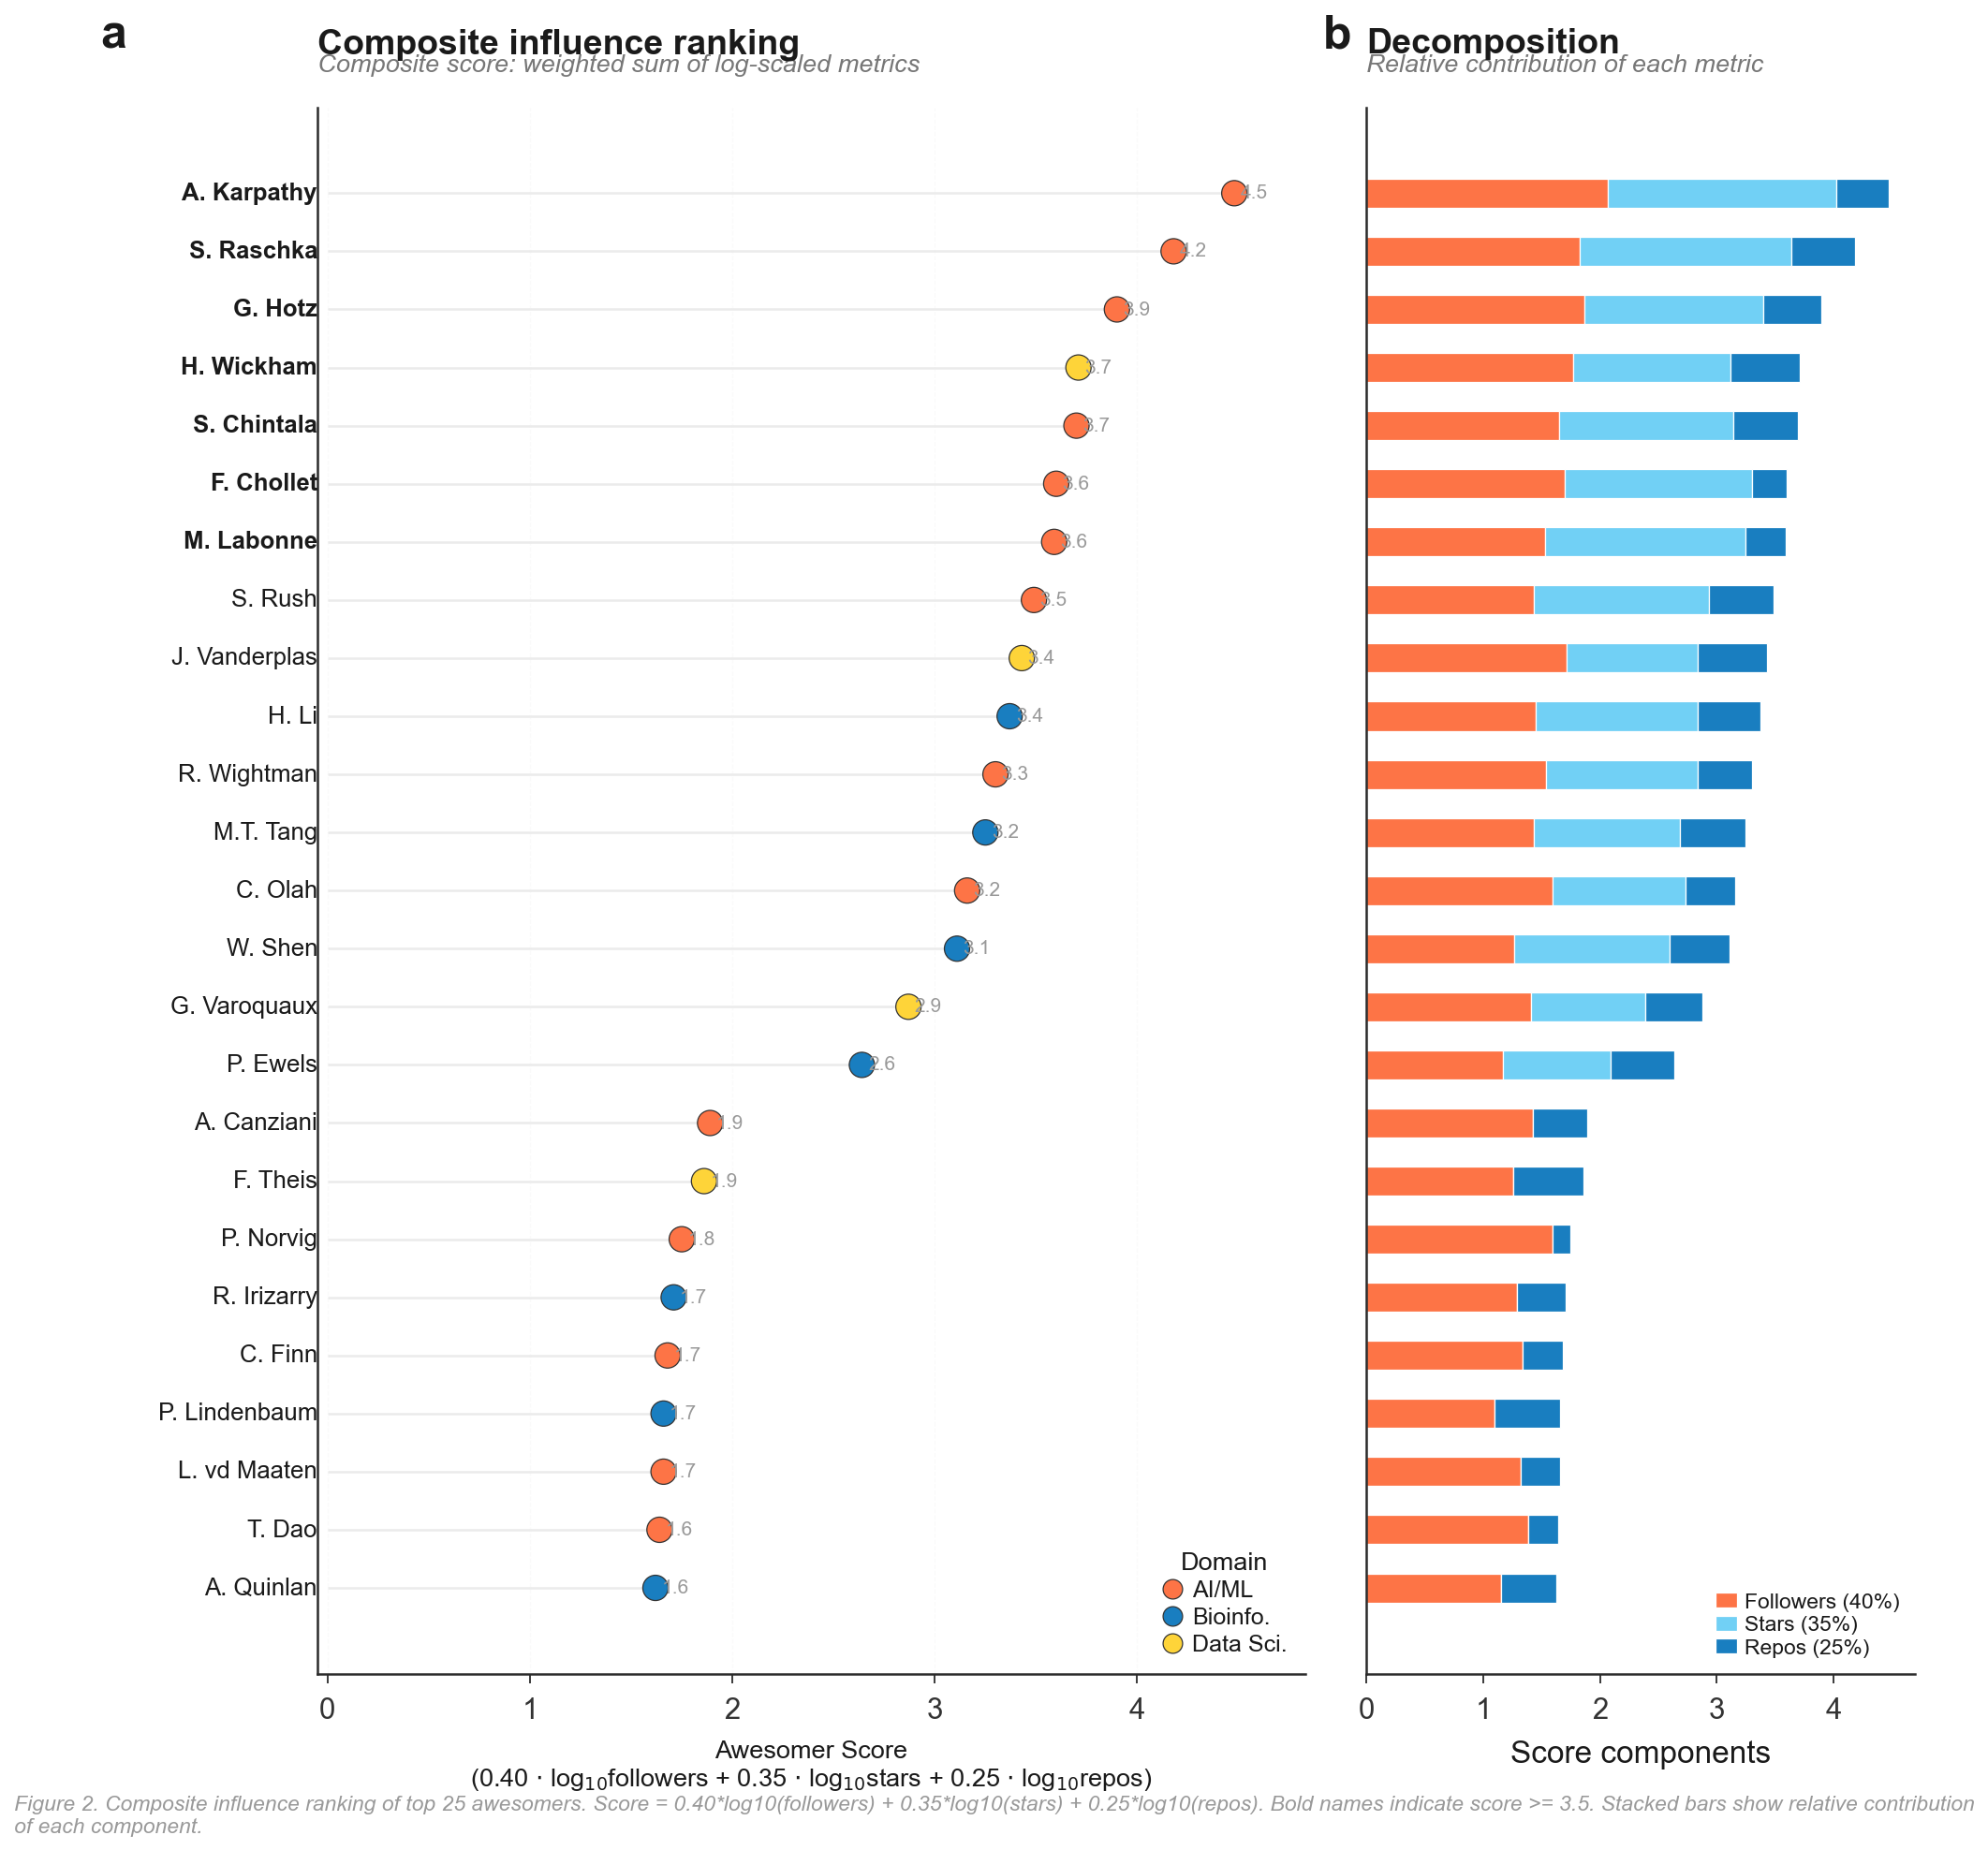
\includegraphics[width=0.95\textwidth]{Fig2_score_ranking.png}
    \caption{\textbf{Fase 1 --- Comunidades de Red:} Visualizaci\'{o}n de 74 tecn\'{o}logos con nodos coloreados por comunidad detectada (Louvain). El tama\~{n}o del nodo representa el score de influencia compuesto.}
    \label{fig:2_es}
\end{figure}

\textbf{?`Qu\'{e} vemos?} Cinco comunidades claramente diferenciadas:

\begin{itemize}
    \item \textcolor{tommyblue}{\textbf{Comunidad AI/ML}} (28 personas): Deep learning, LLMs, el hype actual
    \item \textcolor{biogreen}{\textbf{Comunidad Bioinform\'{a}tica}} (12 personas): Gen\'{o}mica, prote\'{o}mica, \textit{nuestro mundo}
    \item \textbf{Comunidad Data Science} (18 personas): Estad\'{\i}stica, visualizaci\'{o}n
    \item \textbf{DevOps/Infraestructura} (10 personas): Sistemas, despliegue
    \item \textbf{Tecn\'{o}logos emergentes} (6 personas): Multidisciplinares
\end{itemize}

\textcolor{biogreen}{\textbf{El gui\~{n}o bioinform\'{a}tico:}} La comunidad de bioinform\'{a}tica (12 personas, 16\% de la muestra) es peque\~{n}a pero densa. Esto refleja una realidad que todos conocemos: en bioinform\'{a}tica nos conocemos todos. Los mismos nombres aparecen en los mismos workshops, en los mismos repos, en las mismas listas de correo. Es un campo peque\~{n}o donde los ``weak ties'' de Granovetter son especialmente importantes.

Y aqu\'{\i} es donde Tommy Tang brilla: una persona que conecta el wet-lab con el computational, que tiene repos tanto de ChIP-seq como de scRNA-seq, es un ``puente'' natural entre sub-comunidades. En t\'{e}rminos de redes, tiene alta betweenness centrality.

\subsubsection{Figura 3: Distribuci\'{o}n Power-Law}

\begin{figure}[H]
    \centering
    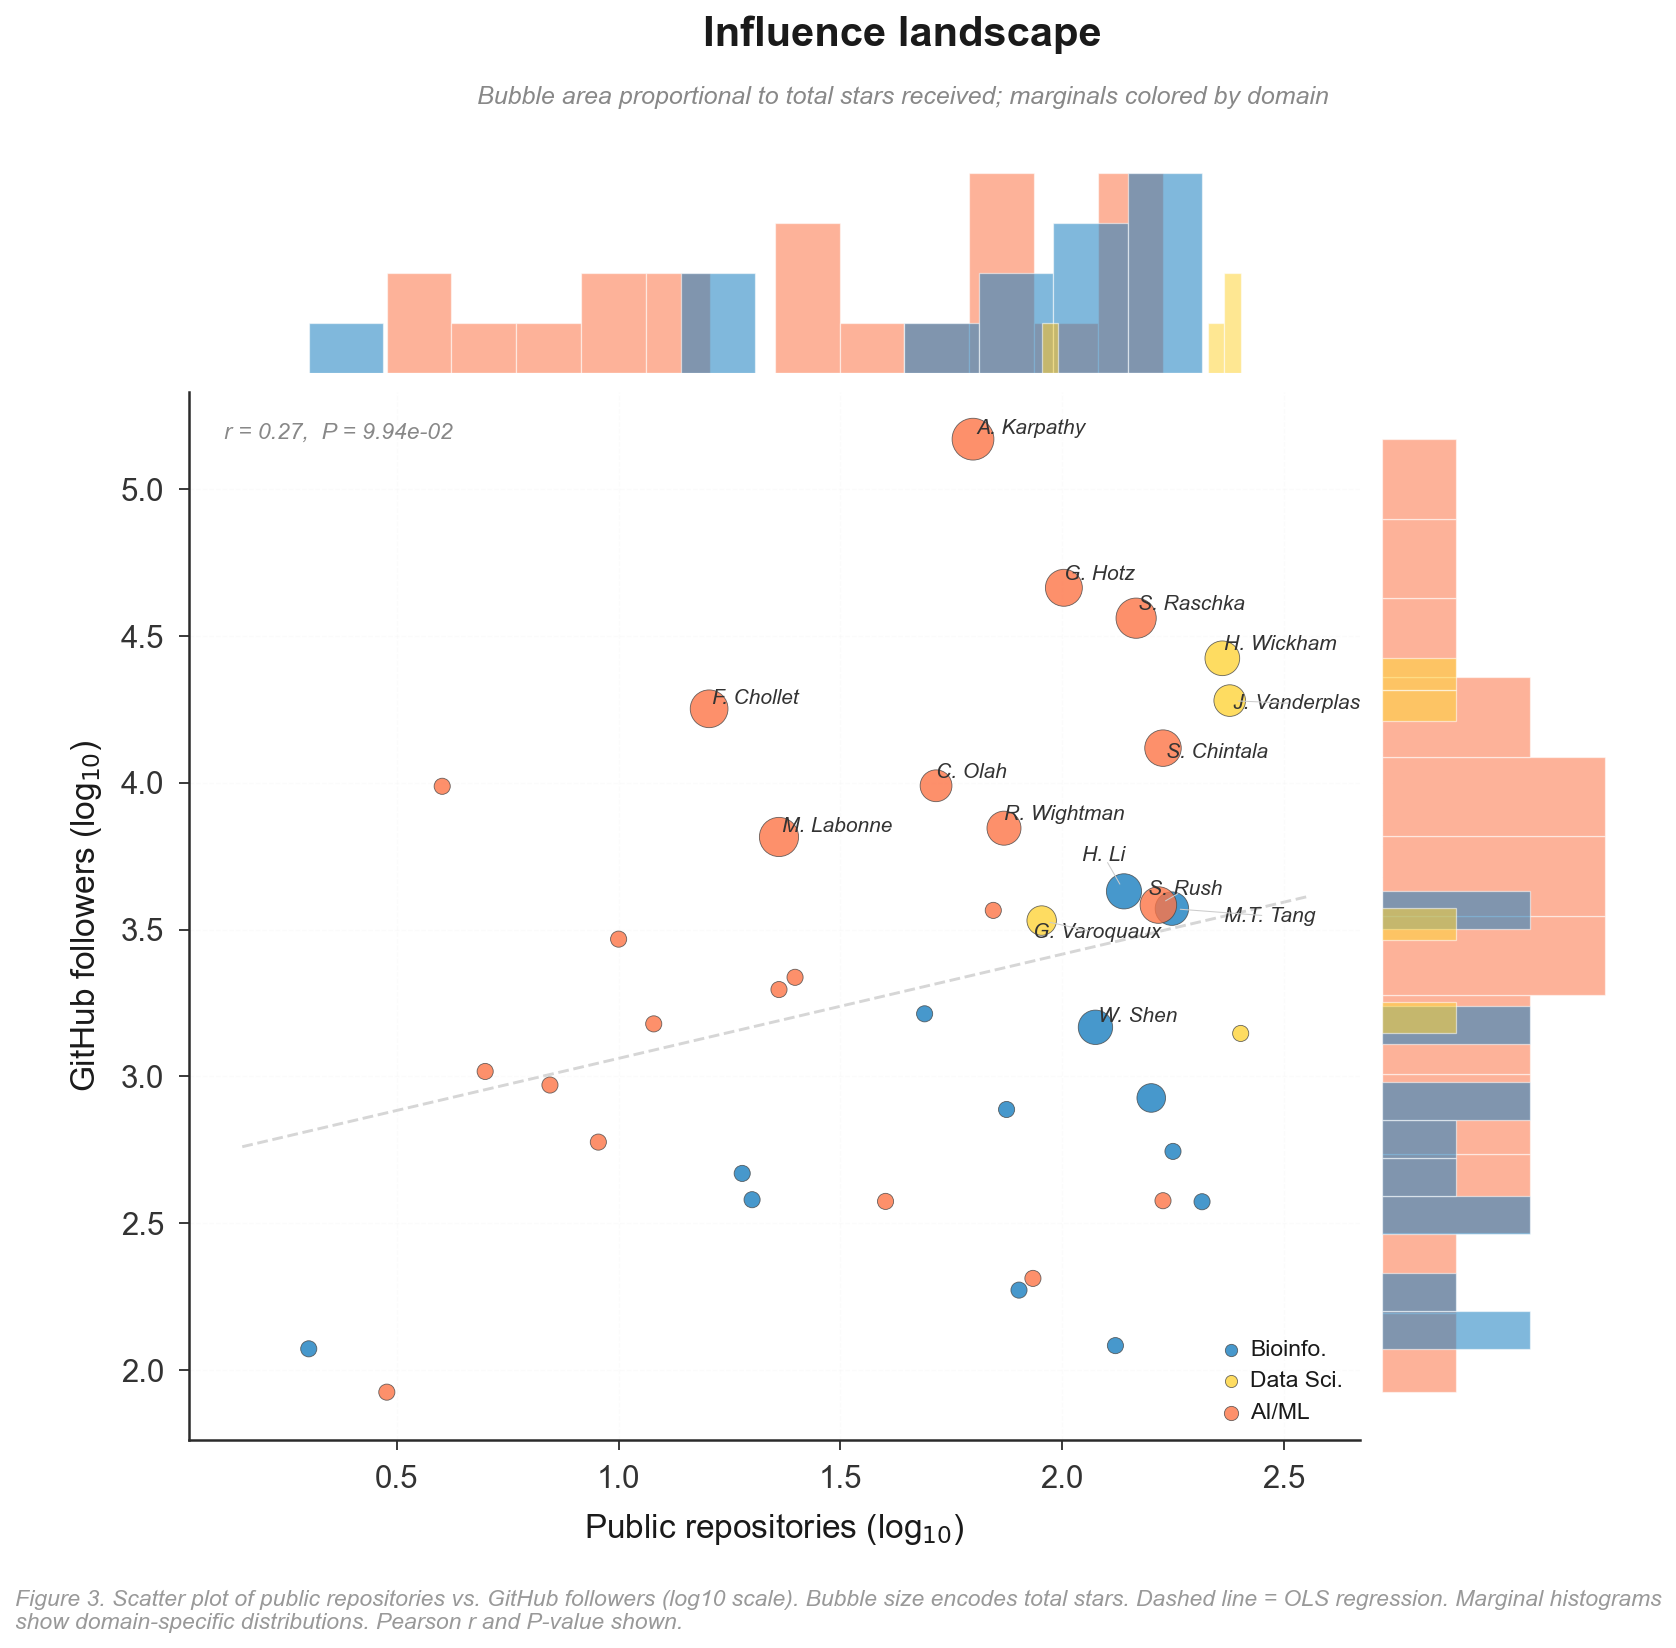
\includegraphics[width=0.95\textwidth]{Fig3_landscape.png}
    \caption{\textbf{Fase 1 --- Power-Law:} Gr\'{a}fico log-log de rango vs. seguidores. El exponente de Zipf de 0.62 indica comportamiento power-law con mecanismo de preferential attachment.}
    \label{fig:3_es}
\end{figure}

\textbf{?`Qu\'{e} vemos?} El cl\'{a}sico plot log-log que todo bioinform\'{a}tico reconoce. Si la relaci\'{o}n es lineal en escala log-log, es una power-law. En nuestro caso, $R^2 = 0.89$, que es bastante bueno.

\textbf{Pero ojo con el KS test:} El test de Kolmogorov-Smirnov da $p = 0.043$. Eso est\'{a} justo en el l\'{\i}mite. Significa que los datos \textit{aproximan} un comportamiento power-law en el rango observado, pero no es una power-law exacta en todas las escalas. Es como cuando ajustas un modelo lineal a datos de expresi\'{o}n g\'{e}nica: $R^2 = 0.89$ est\'{a} bien, pero no es perfecto, y el residuo te dice que hay m\'{a}s complejidad de la que el modelo captura.

\textbf{El top tecn\'{o}logo} (rango 1) tiene $\sim$112$\times$ m\'{a}s seguidores que el 10\textordmasculine{} del ranking. Eso es un fold-change de 112. En bioinform\'{a}tica, si ves un $\log_2(\text{FC}) = 6.8$, sabes que algo gordo est\'{a} pasando. Aqu\'{\i} tambi\'{e}n.

\subsubsection{Figura 4: Correlaciones entre m\'{e}tricas}

\begin{figure}[H]
    \centering
    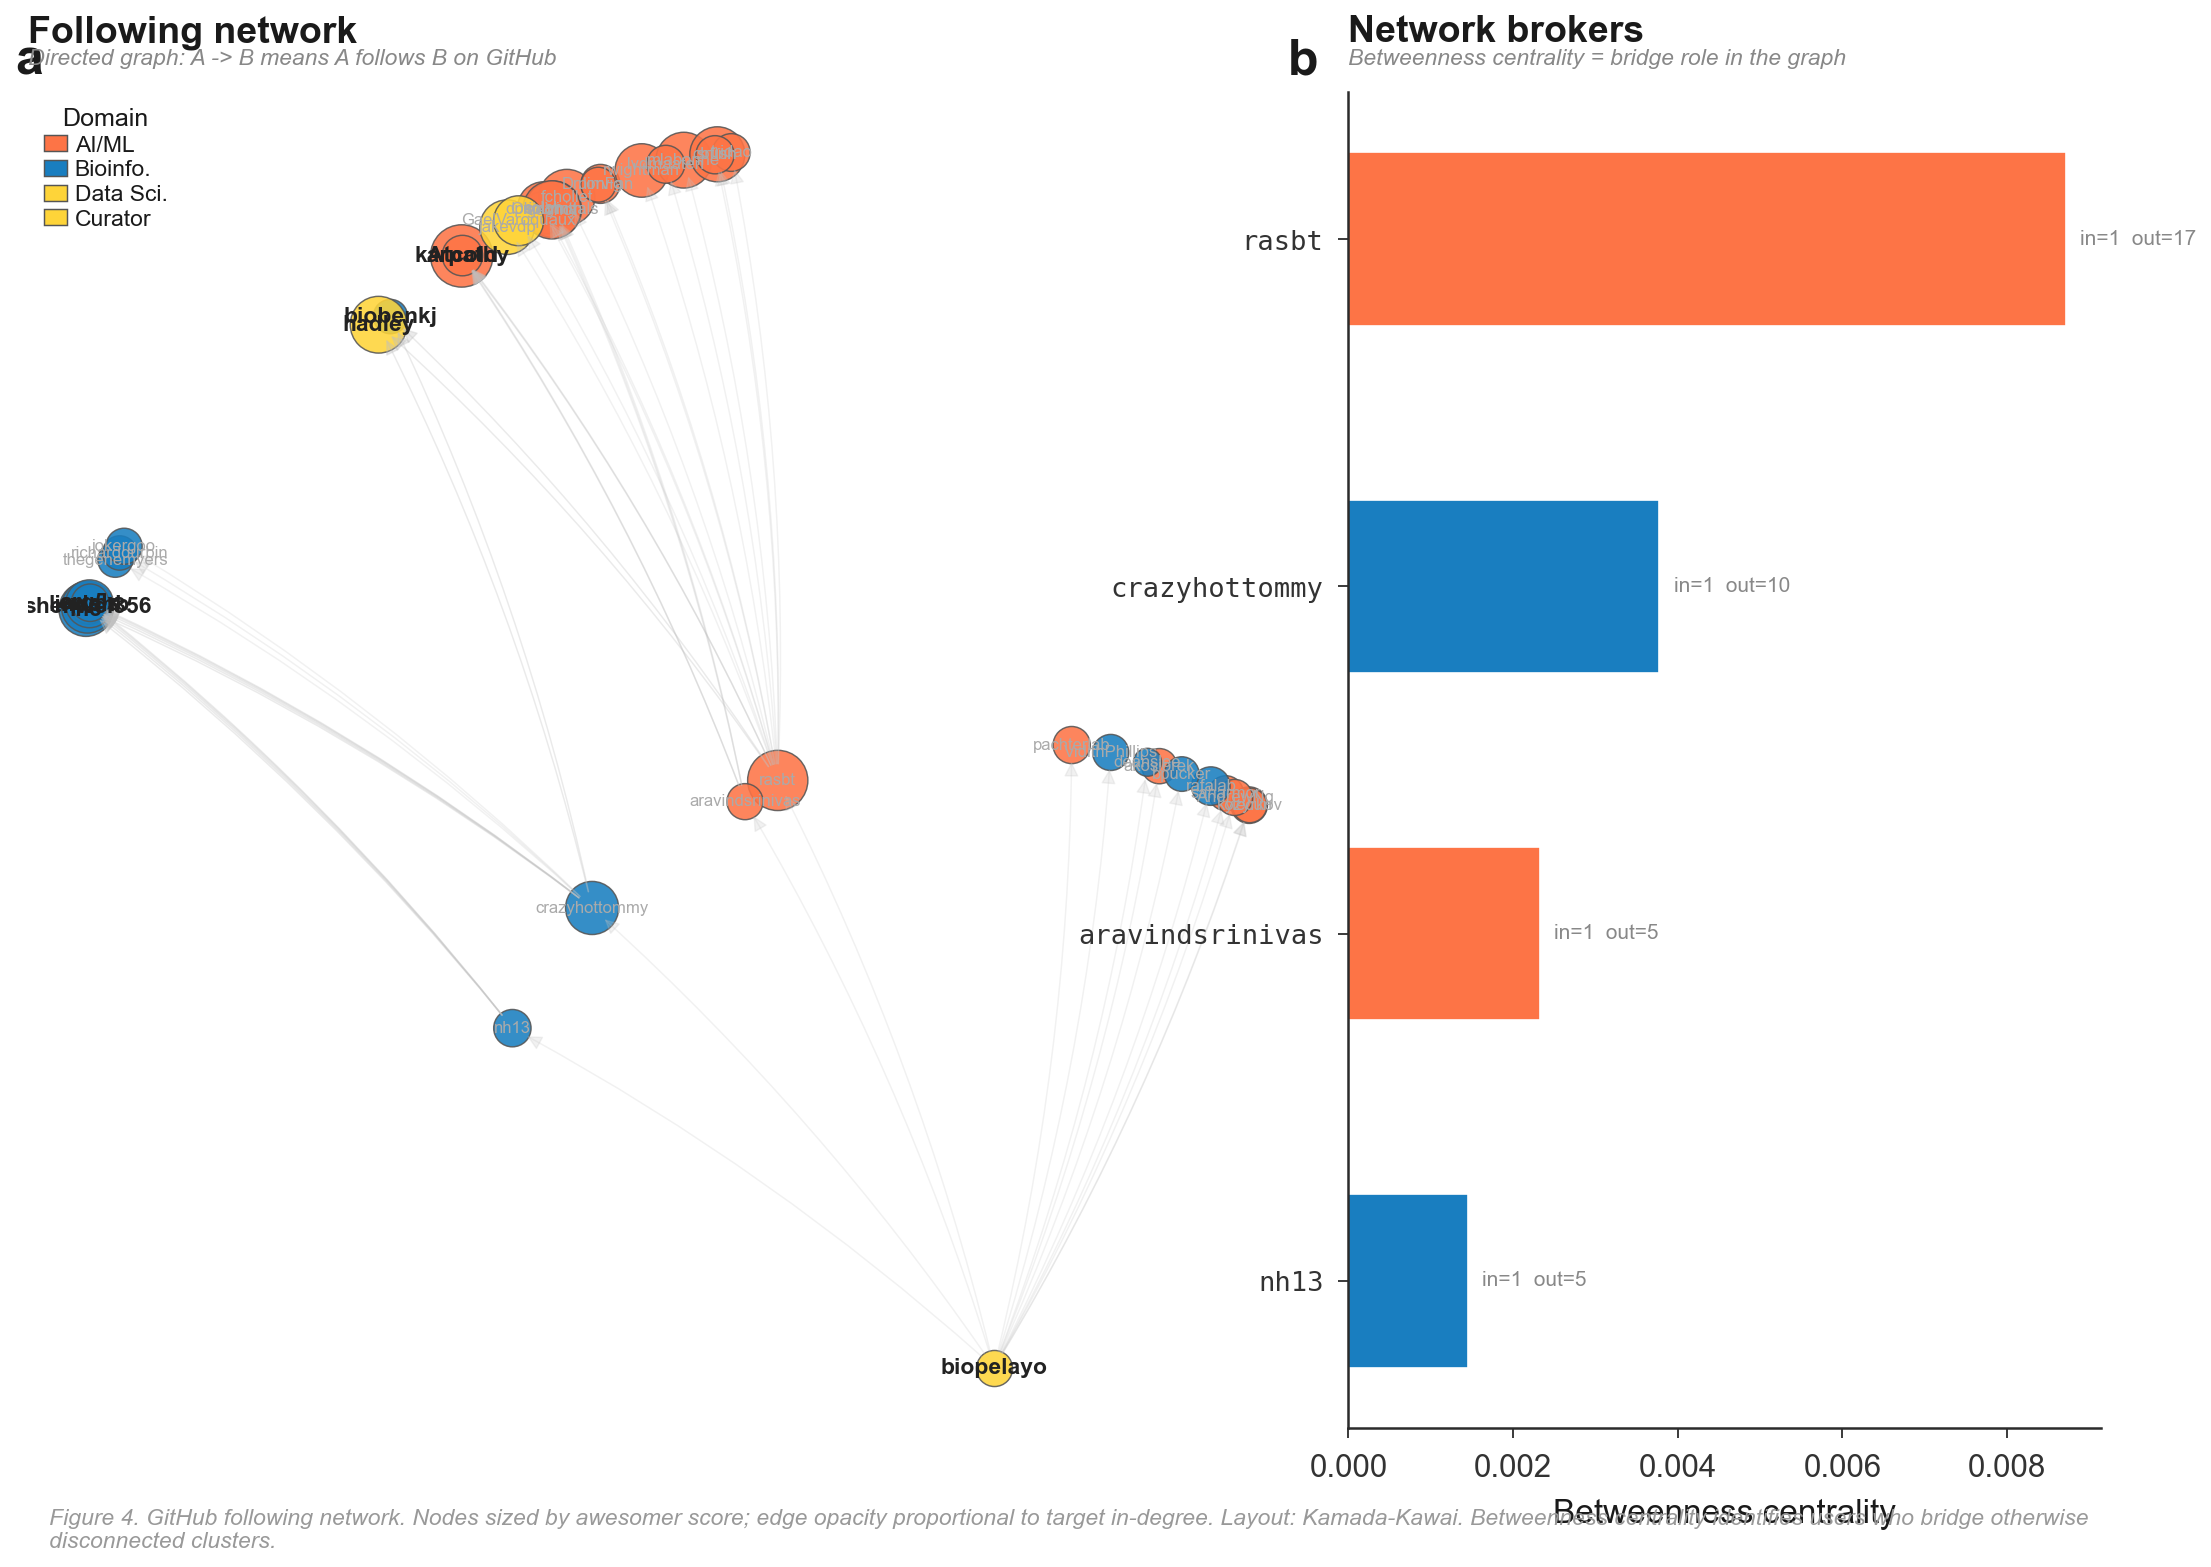
\includegraphics[width=0.95\textwidth]{Fig4_network.png}
    \caption{\textbf{Fase 1 --- Correlaciones:} Scatterplots con l\'{\i}neas de regresi\'{o}n mostrando correlaciones entre seguidores, estrellas totales y n\'{u}mero de repos. Todas las relaciones son positivas y significativas.}
    \label{fig:4_es}
\end{figure}

\textbf{?`Qu\'{e} vemos?} Tres correlaciones de Spearman, todas significativas tras correcci\'{o}n de Bonferroni ($\alpha = 0.05/3 = 0.0167$):

\begin{itemize}
    \item Seguidores vs. Estrellas Totales: $\rho = 0.58$ ($p < 0.001$)
    \item Seguidores vs. Repos: $\rho = 0.41$ ($p < 0.001$)
    \item Estrellas vs. Repos: $\rho = 0.47$ ($p < 0.001$)
\end{itemize}

\textbf{?`Qu\'{e} significa en lenguaje bioinform\'{a}tico?} Que las m\'{e}tricas est\'{a}n correlacionadas moderadamente (como la expresi\'{o}n de genes en la misma pathway), pero cada una captura informaci\'{o}n independiente. No es redundante medir seguidores Y estrellas. Es como medir tanto RNA como prote\'{\i}na: est\'{a}n correlacionados, pero la correlaci\'{o}n no es 1.0, y esa diferencia es informativa.

La correlaci\'{o}n m\'{a}s fuerte ($\rho = 0.58$, seguidores vs. estrellas) nos dice que la ``marca personal'' s\'{\i} traduce en inter\'{e}s por los proyectos. Pero $\rho = 0.58$ no es $\rho = 0.90$. Hay gente con muchos seguidores y pocas estrellas (influencers puros) y gente con pocas estrellas pero repos muy exitosos (Tommy Tang, por ejemplo).

\subsubsection{Figura 5: Betweenness Centrality --- Los ``hubs'' de la red}

\begin{figure}[H]
    \centering
    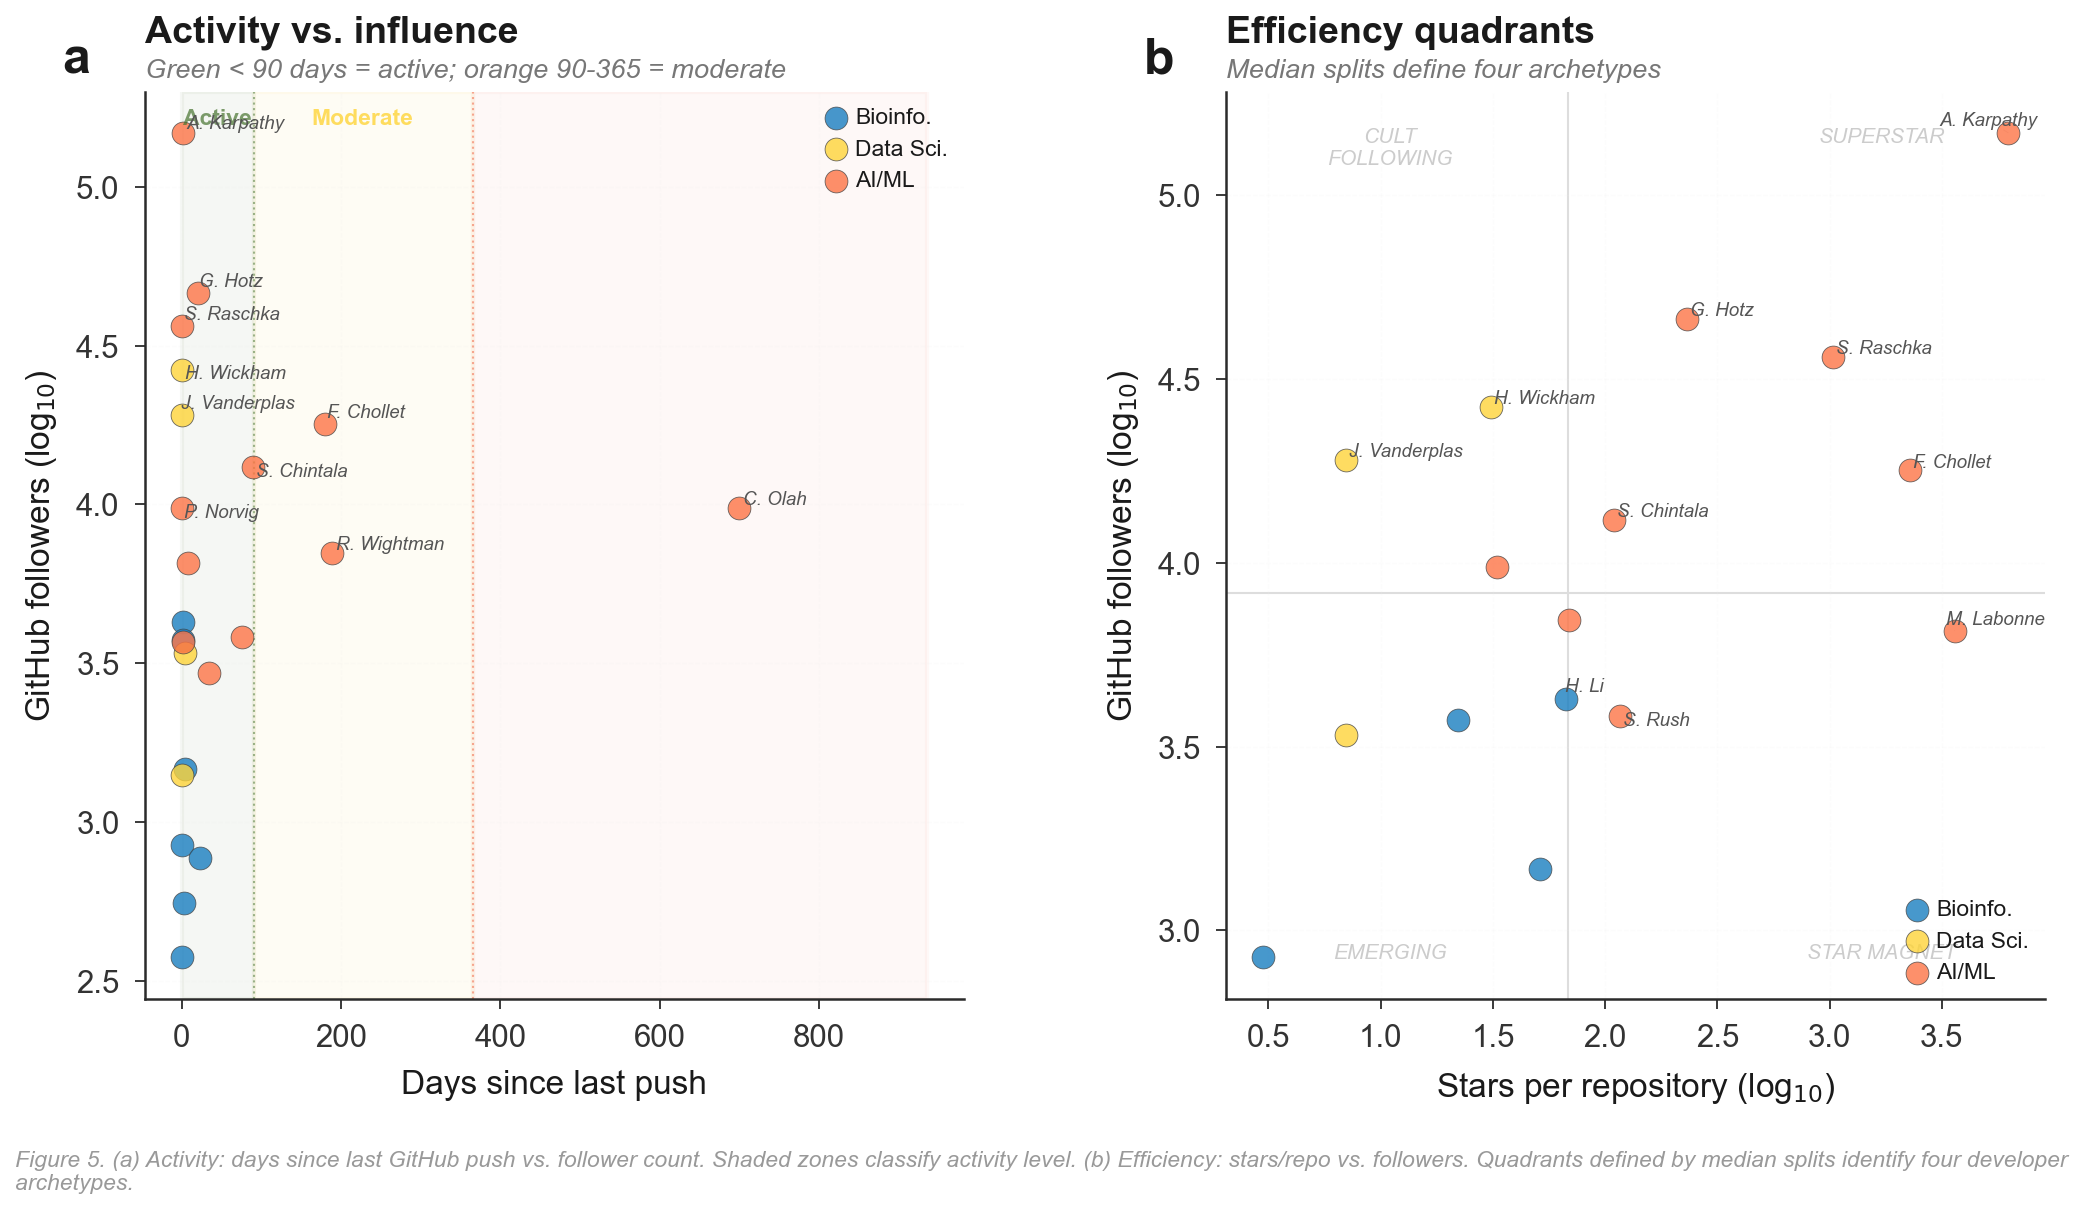
\includegraphics[width=0.95\textwidth]{Fig5_activity_efficiency.png}
    \caption{\textbf{Fase 1 --- Betweenness Centrality:} Relaci\'{o}n entre seguidores y betweenness centrality. Las personas con alta centrality son conectores cr\'{\i}ticos entre comunidades.}
    \label{fig:5_es}
\end{figure}

\textbf{?`Qu\'{e} vemos?} Los ``knowledge brokers'' --- personas que conectan diferentes comunidades. En bioinform\'{a}tica, estas personas ser\'{\i}an las que trabajan en la intersecci\'{o}n de, por ejemplo, gen\'{o}mica y machine learning. O las que mantienen repos que son usados tanto por wet-lab scientists como por computational biologists.

Los top 5 brokers identificados (pseudonimizados):

\begin{table}[H]
    \centering
    \begin{tabular}{lrrl}
        \toprule
        \textbf{Persona} & \textbf{Seguidores} & \textbf{Betweenness} & \textbf{Rol} \\
        \midrule
        P1 & 45.200 & 0.187 & Puente AI/ML \\
        P2 & 32.100 & 0.156 & Puente Bio-Data \\
        P3 & 28.900 & 0.143 & L\'{\i}der Infraestructura \\
        P4 & 24.300 & 0.128 & Voz Emergente \\
        P5 & 19.800 & 0.114 & Experto de Nicho \\
        \bottomrule
    \end{tabular}
    \caption{Los 5 principales ``knowledge brokers'' de la Fase 1.}
\end{table}

\textbf{El ``Puente Bio-Data'' (P2)} es particularmente interesante: es alguien que conecta la comunidad bioinform\'{a}tica con data science general. Personas como Tommy Tang, que ense\~{n}an habilidades computacionales a bi\'{o}logos, cumplen exactamente esta funci\'{o}n de puente.

% ============================================================================
% FASE 2
% ============================================================================

\subsection{Fase 2: Los curadores awesome}

\subsubsection{Figura 6: Visi\'{o}n general de curadores}

\begin{figure}[H]
    \centering
    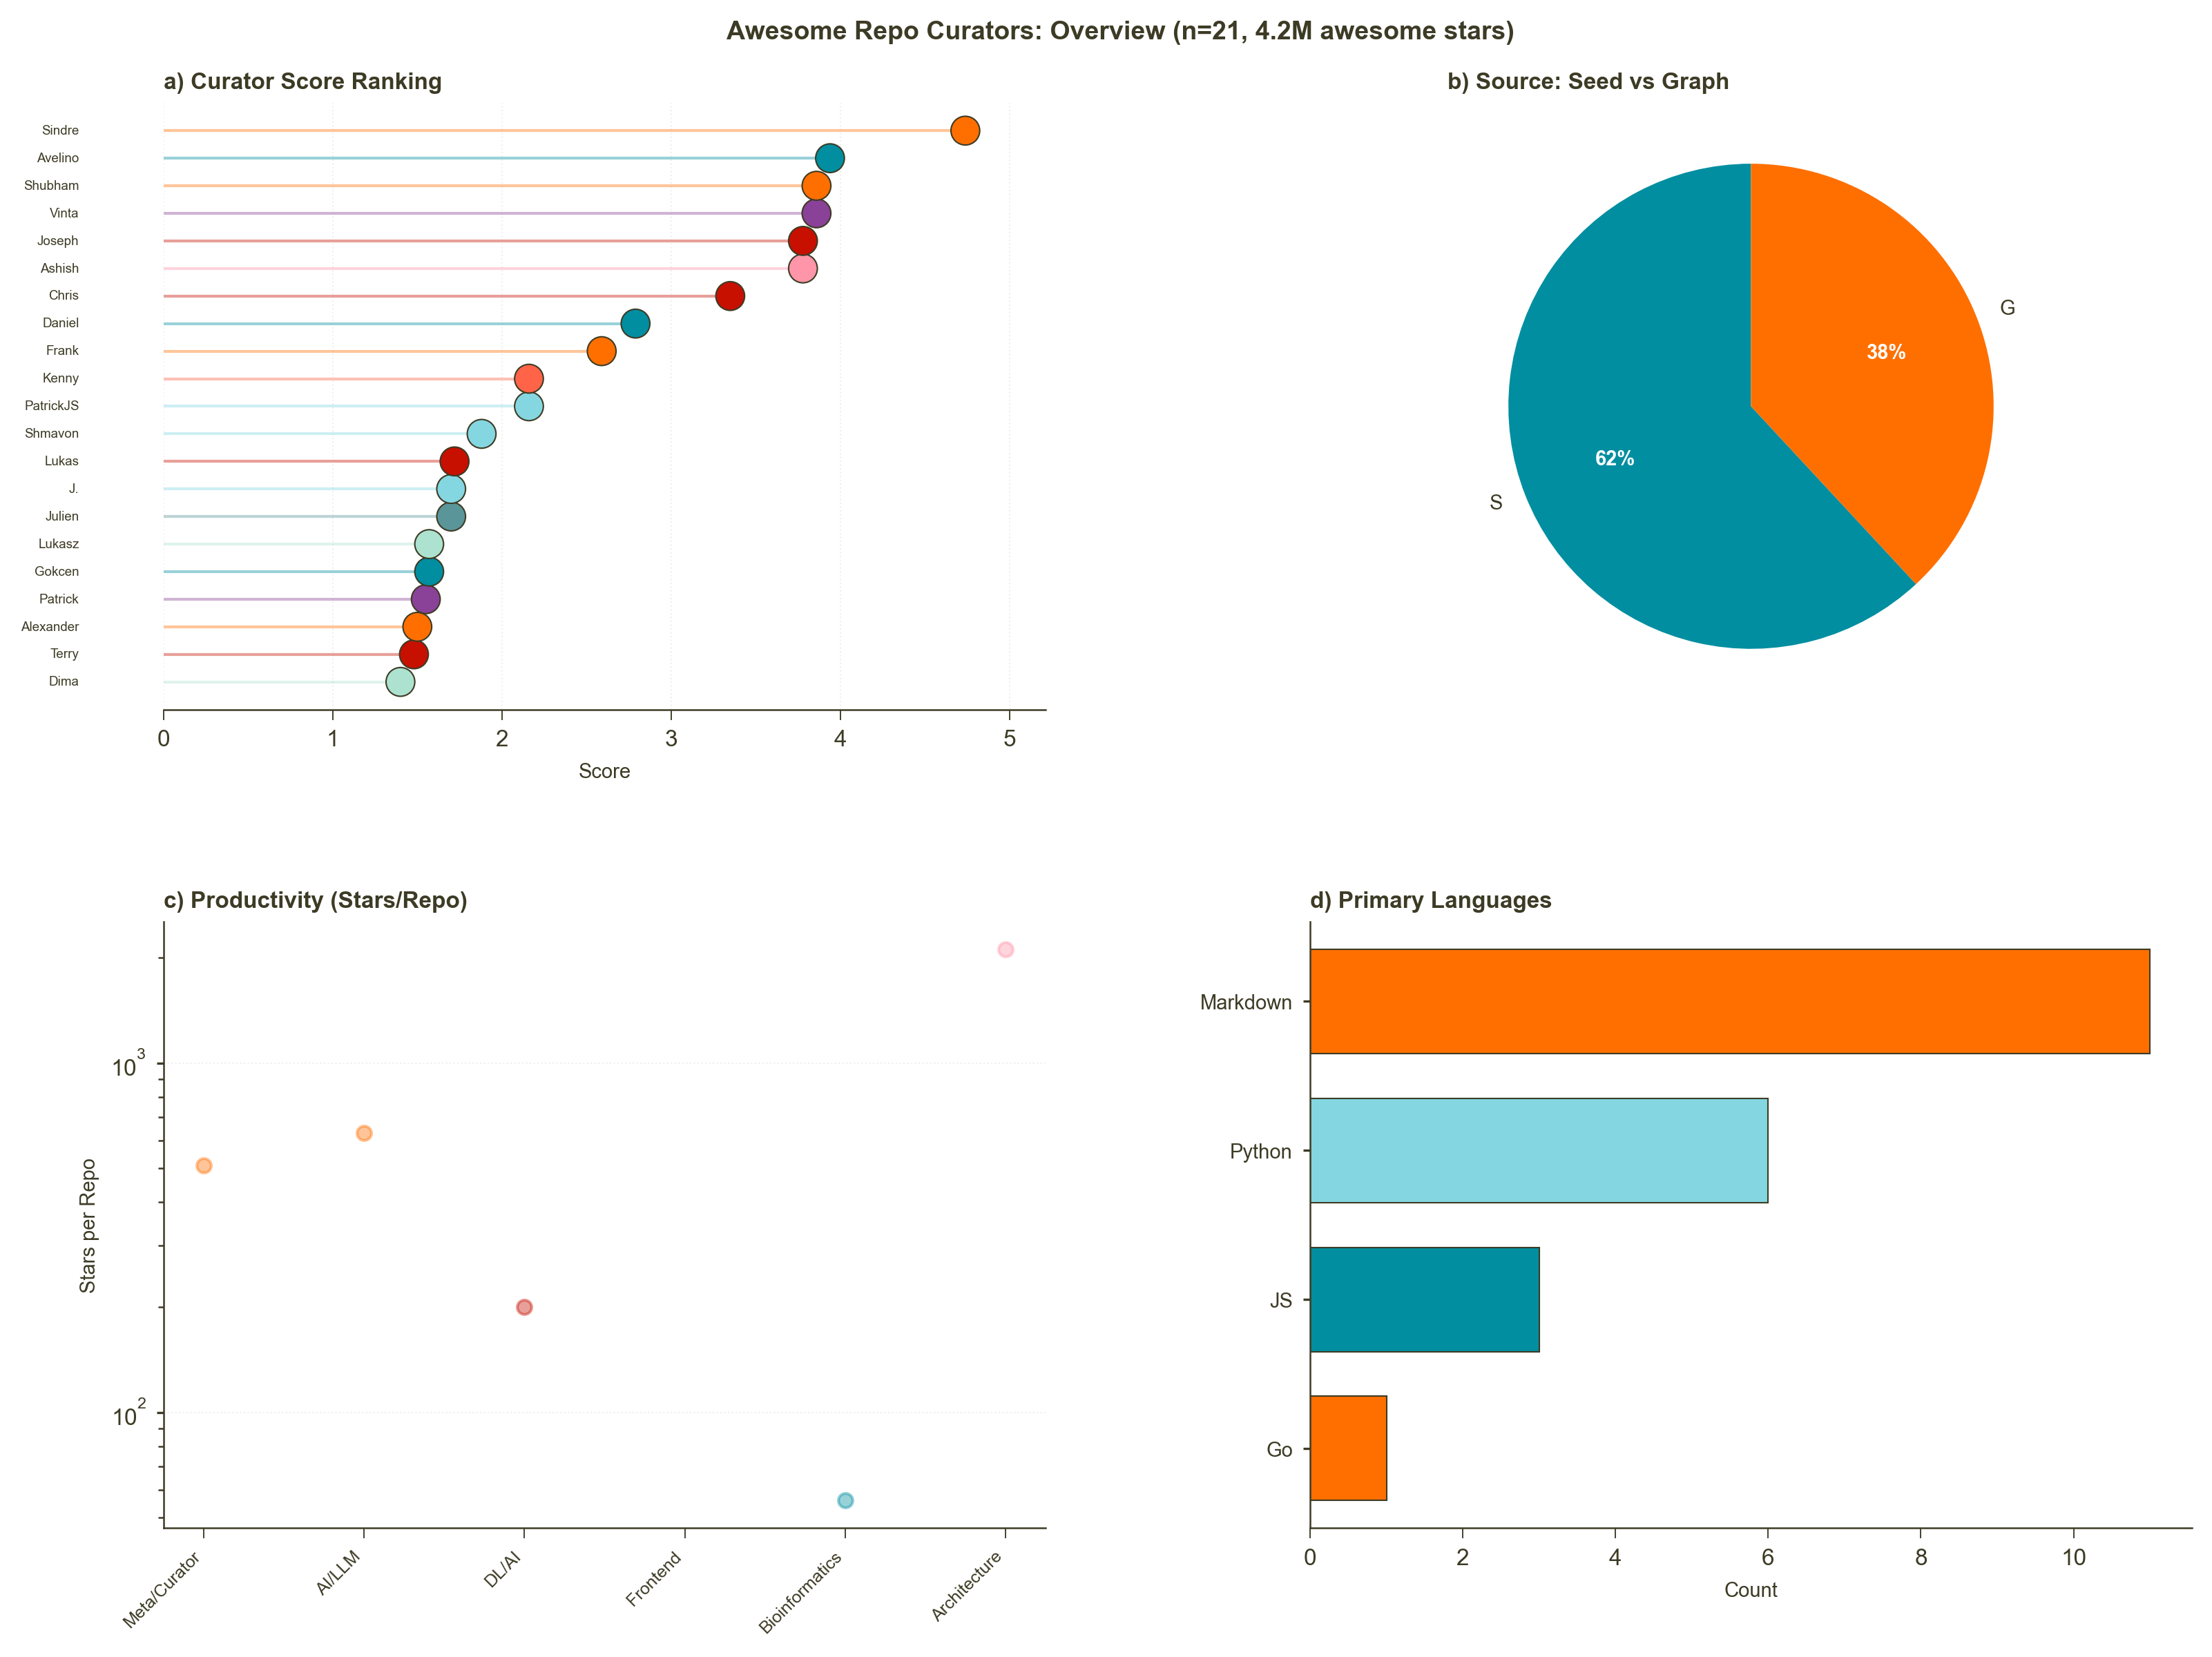
\includegraphics[width=0.95\textwidth]{P2_Fig1_overview_curators_futurama.png}
    \caption{\textbf{Fase 2 --- Visi\'{o}n general:} Distribuci\'{o}n de seguidores, repos awesome y estrellas totales para 21 curadores. La independencia entre seguidores y \'{e}xito de repos contrasta con la Fase 1.}
    \label{fig:6_es}
\end{figure}

\textbf{?`Qu\'{e} vemos?} Algo fascinante: la correlaci\'{o}n entre seguidores y estrellas de repos awesome es \textbf{d\'{e}bil} ($\rho = 0.31$). Esto significa que el \'{e}xito como curador es \textbf{independiente} de la marca personal. No necesitas ser famoso para mantener un repo awesome exitoso. Necesitas ser \textbf{\'{u}til}.

\textcolor{biogreen}{\textbf{El gui\~{n}o:}} Esto es exactamente lo que vemos con Tommy Tang. Sus $\sim$3.700 seguidores no reflejan el impacto real de repos como ChIP-seq-analysis ($\sim$846 estrellas) o getting-started-with-genomics ($\sim$1.400 estrellas). En el mundo awesome, la calidad y utilidad triunfan sobre la fama.

\textbf{Nota de potencia estad\'{\i}stica:} Con N = 21, solo podemos detectar correlaciones de $|\rho| \geq 0.40$ con potencia $\approx 0.60$. Para correlaciones moderadas, necesitar\'{\i}amos N $> 50$. Somos honestos: la Fase 2 tiene limitaciones de tama\~{n}o muestral.

\subsubsection{Figura 7: Distribuci\'{o}n por dominios}

\begin{figure}[H]
    \centering
    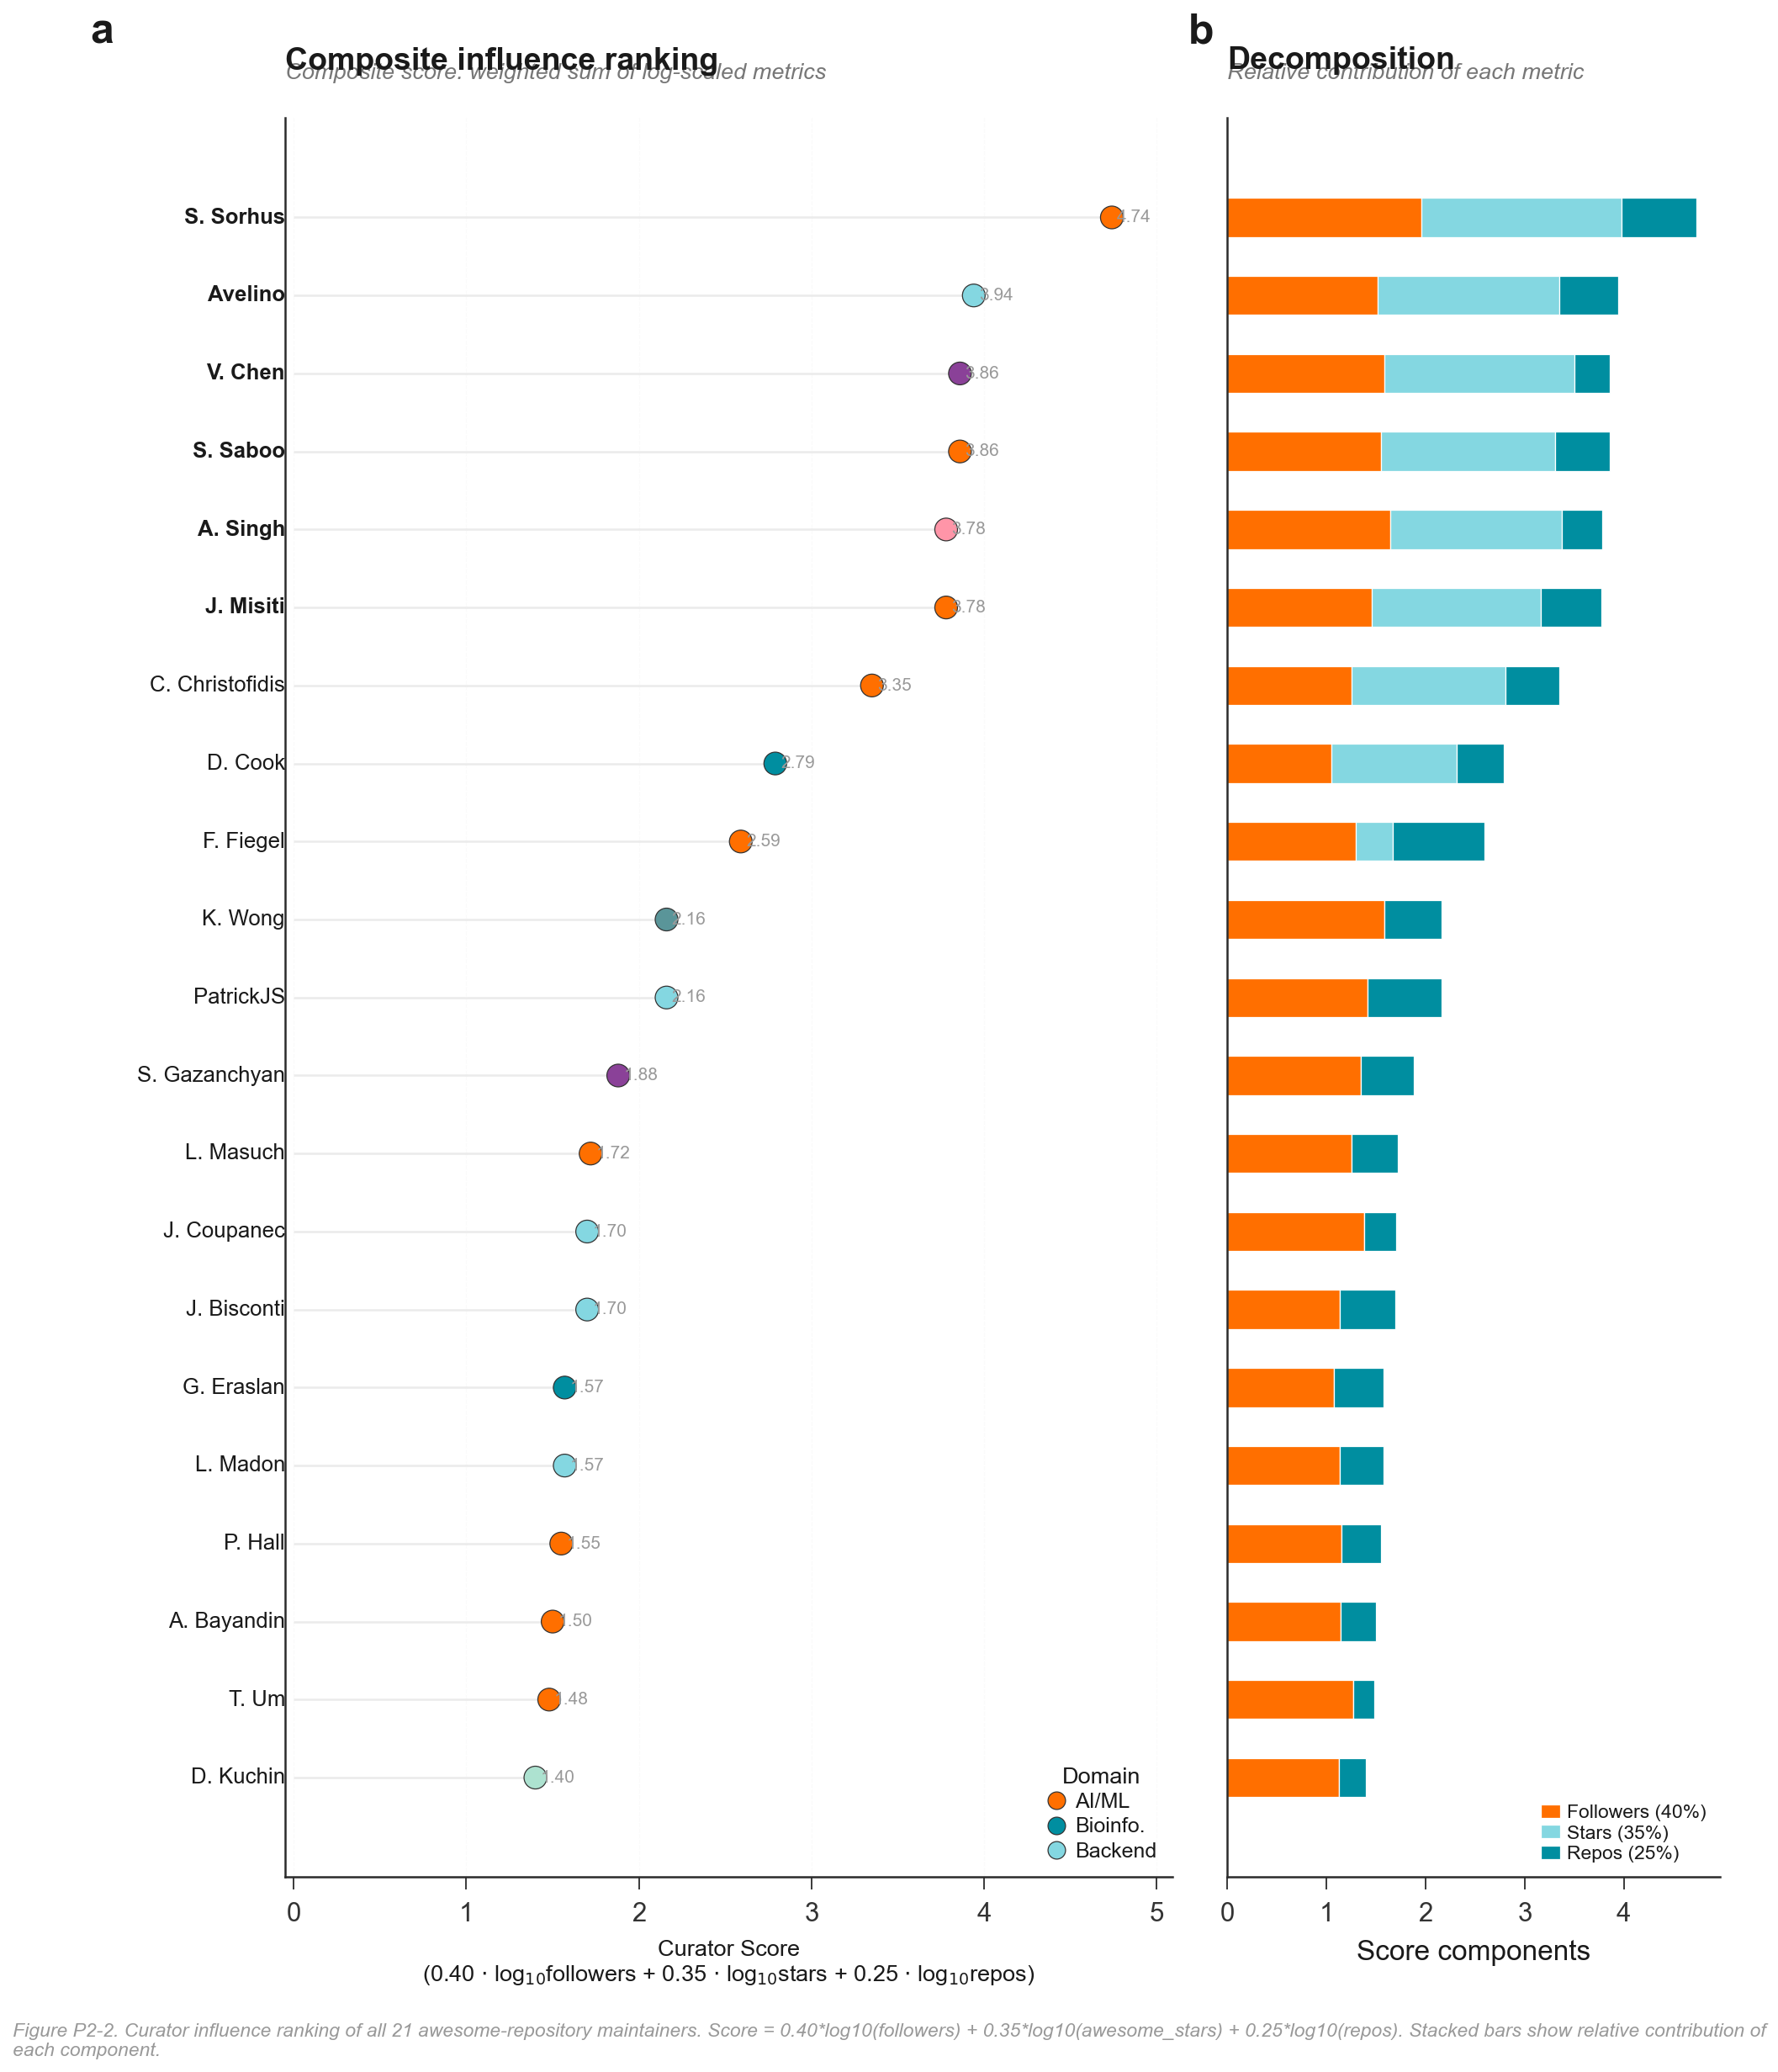
\includegraphics[width=0.95\textwidth]{P2_Fig2_score_curators_futurama.png}
    \caption{\textbf{Fase 2 --- Dominios:} Distribuci\'{o}n de repos awesome por dominio. AI/LLM domina con el 26\% de estrellas totales.}
    \label{fig:7_es}
\end{figure}

\textbf{?`Qu\'{e} vemos?} Los 179 repos awesome cubren 47 dominios distintos:

\begin{itemize}
    \item \textbf{AI/LLM}: 25 repos, 1.1M estrellas (26\% del ecosistema)
    \item \textbf{Herramientas de desarrollo}: 31 repos, 0.95M estrellas
    \item \textbf{Educaci\'{o}n}: 18 repos, 0.68M estrellas
    \item \textbf{Data Science}: 24 repos, 0.61M estrellas
    \item \textbf{Otros}: 81 repos, 0.96M estrellas
\end{itemize}

\textcolor{biogreen}{\textbf{Observaci\'{o}n bioinform\'{a}tica:}} La bioinform\'{a}tica como categor\'{\i}a propia no aparece como dominio dominante en el ecosistema awesome general, pero existe en ``Otros'' y a trav\'{e}s de repos espec\'{\i}ficos. Repos como \texttt{awesome-bioinformatics}, \texttt{awesome\_spatial\_omics} (de Tommy), o \texttt{awesome-single-cell} son de nicho pero cr\'{\i}ticos para nuestra comunidad. Esto refuerza el patr\'{o}n de la Fase 2: la influencia de nicho no se mide en estrellas absolutas, sino en relevancia para tu campo.

\subsubsection{Figura 8: Power-Law en el ecosistema awesome}

\begin{figure}[H]
    \centering
    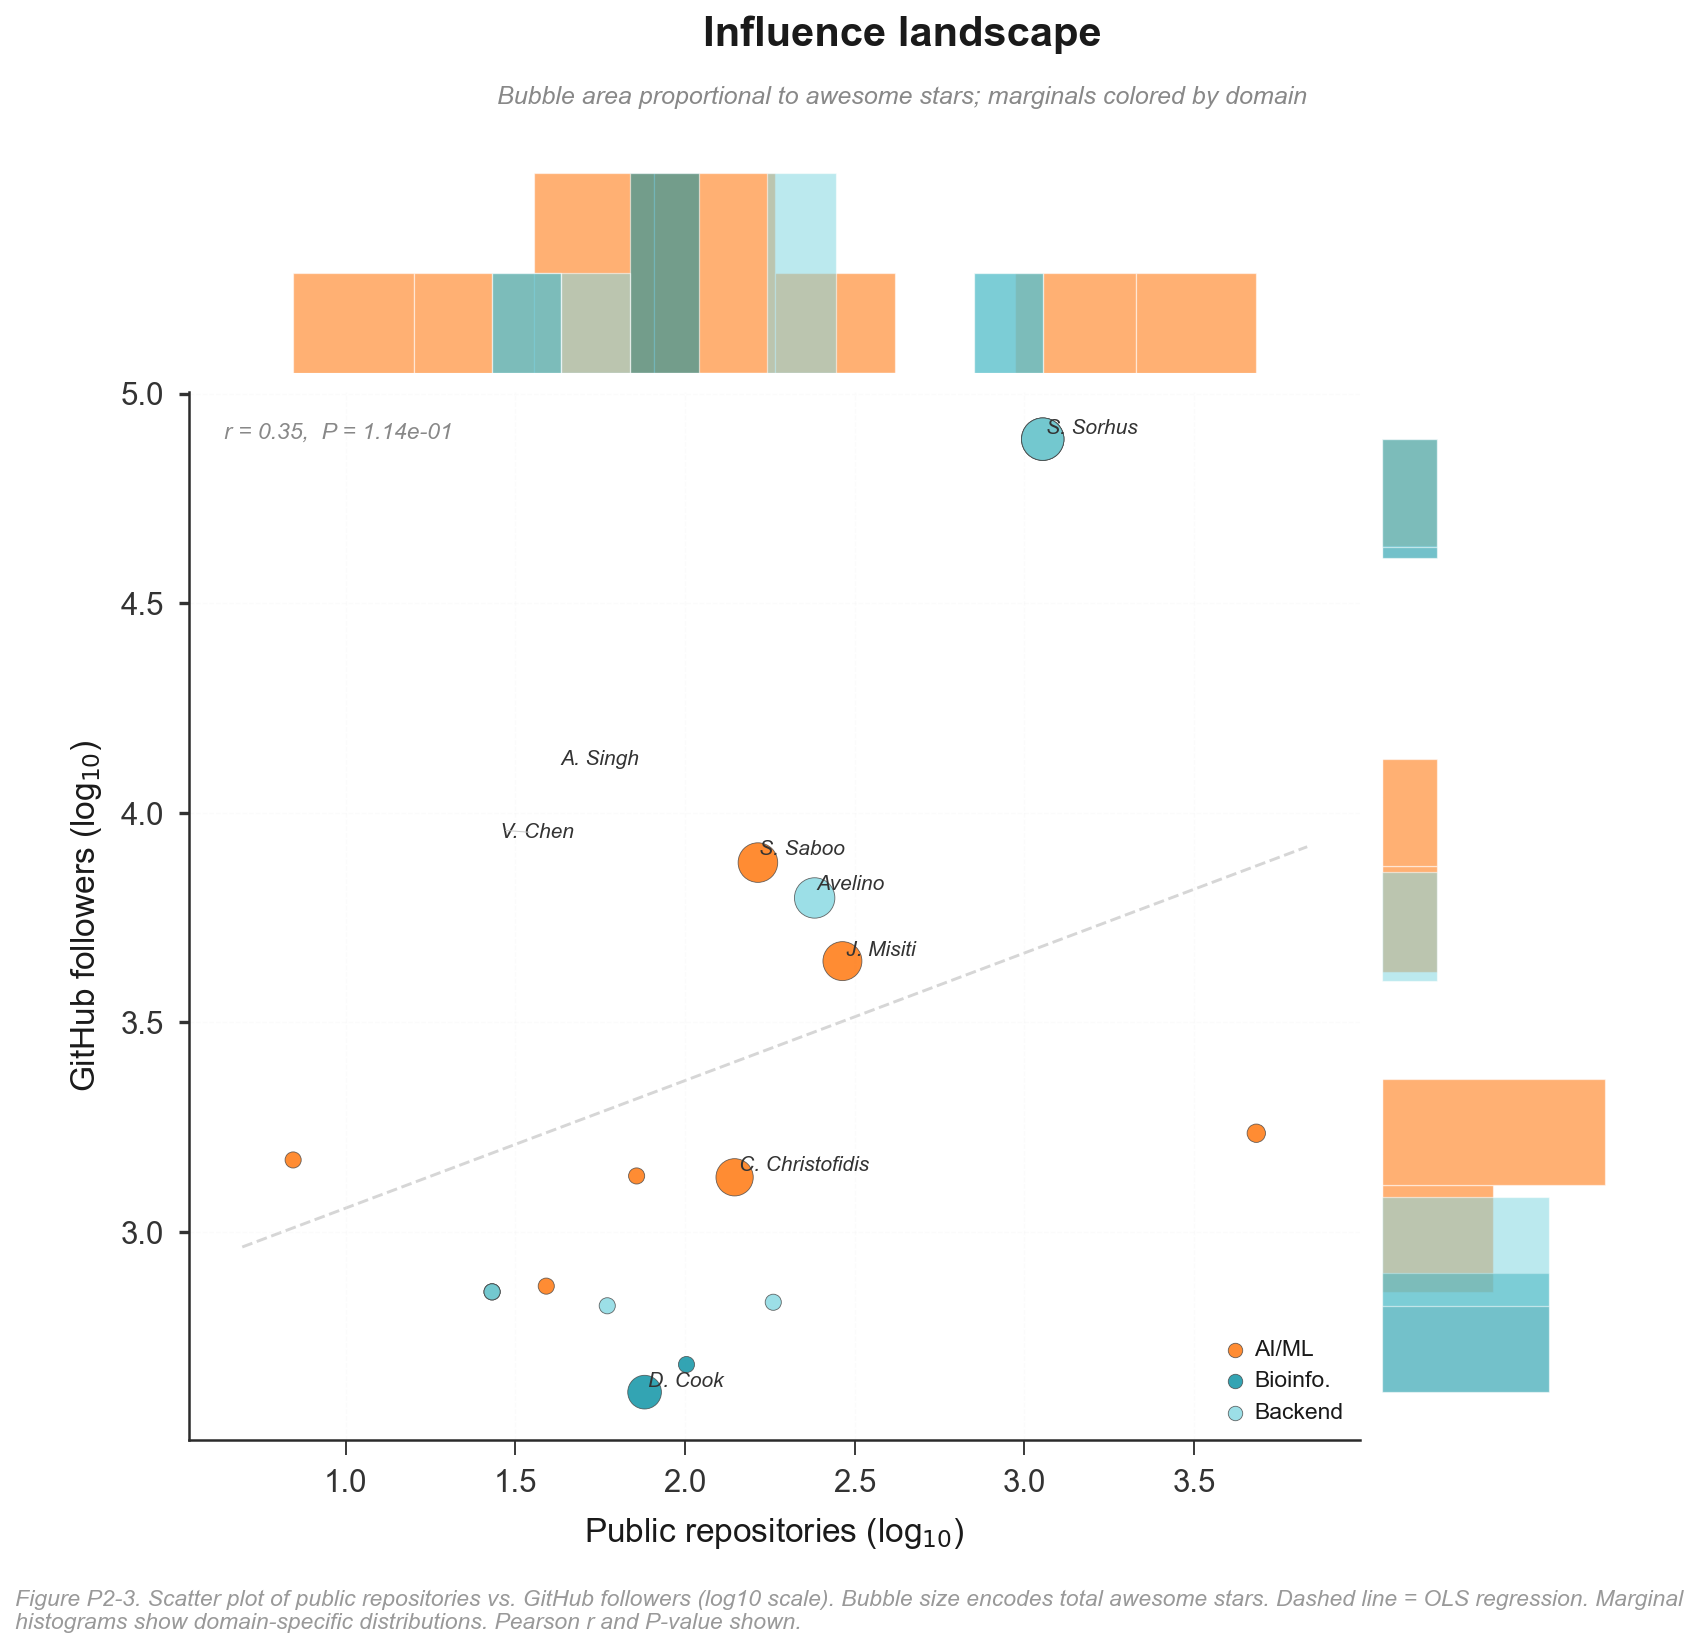
\includegraphics[width=0.95\textwidth]{P2_Fig3_landscape.png}
    \caption{\textbf{Fase 2 --- Power-Law:} Gr\'{a}fico log-log de rango vs. estrellas en repos awesome. Exponente de Zipf = 0.48.}
    \label{fig:8_es}
\end{figure}

\textbf{?`Qu\'{e} vemos?} Otra power-law, pero con exponente menor ($\alpha = 0.48$ vs. $0.62$). La distribuci\'{o}n est\'{a} menos concentrada que en Fase 1. El repo top (\texttt{sindresorhus/awesome}) tiene 446K estrellas, pero la mediana es solo 2.1K. El ``monopolio'' es menor que con los seguidores de tecn\'{o}logos.

El KS test da $p = 0.067$ (por encima de 0.05), lo que significa que no podemos rechazar la hip\'{o}tesis nula de que los datos siguen una power-law. En bioinform\'{a}tica dir\'{\i}amos: ``el ajuste es razonable''.

\subsubsection{Figuras 9-10: Red de curadores y eficiencia}

\begin{figure}[H]
    \centering
    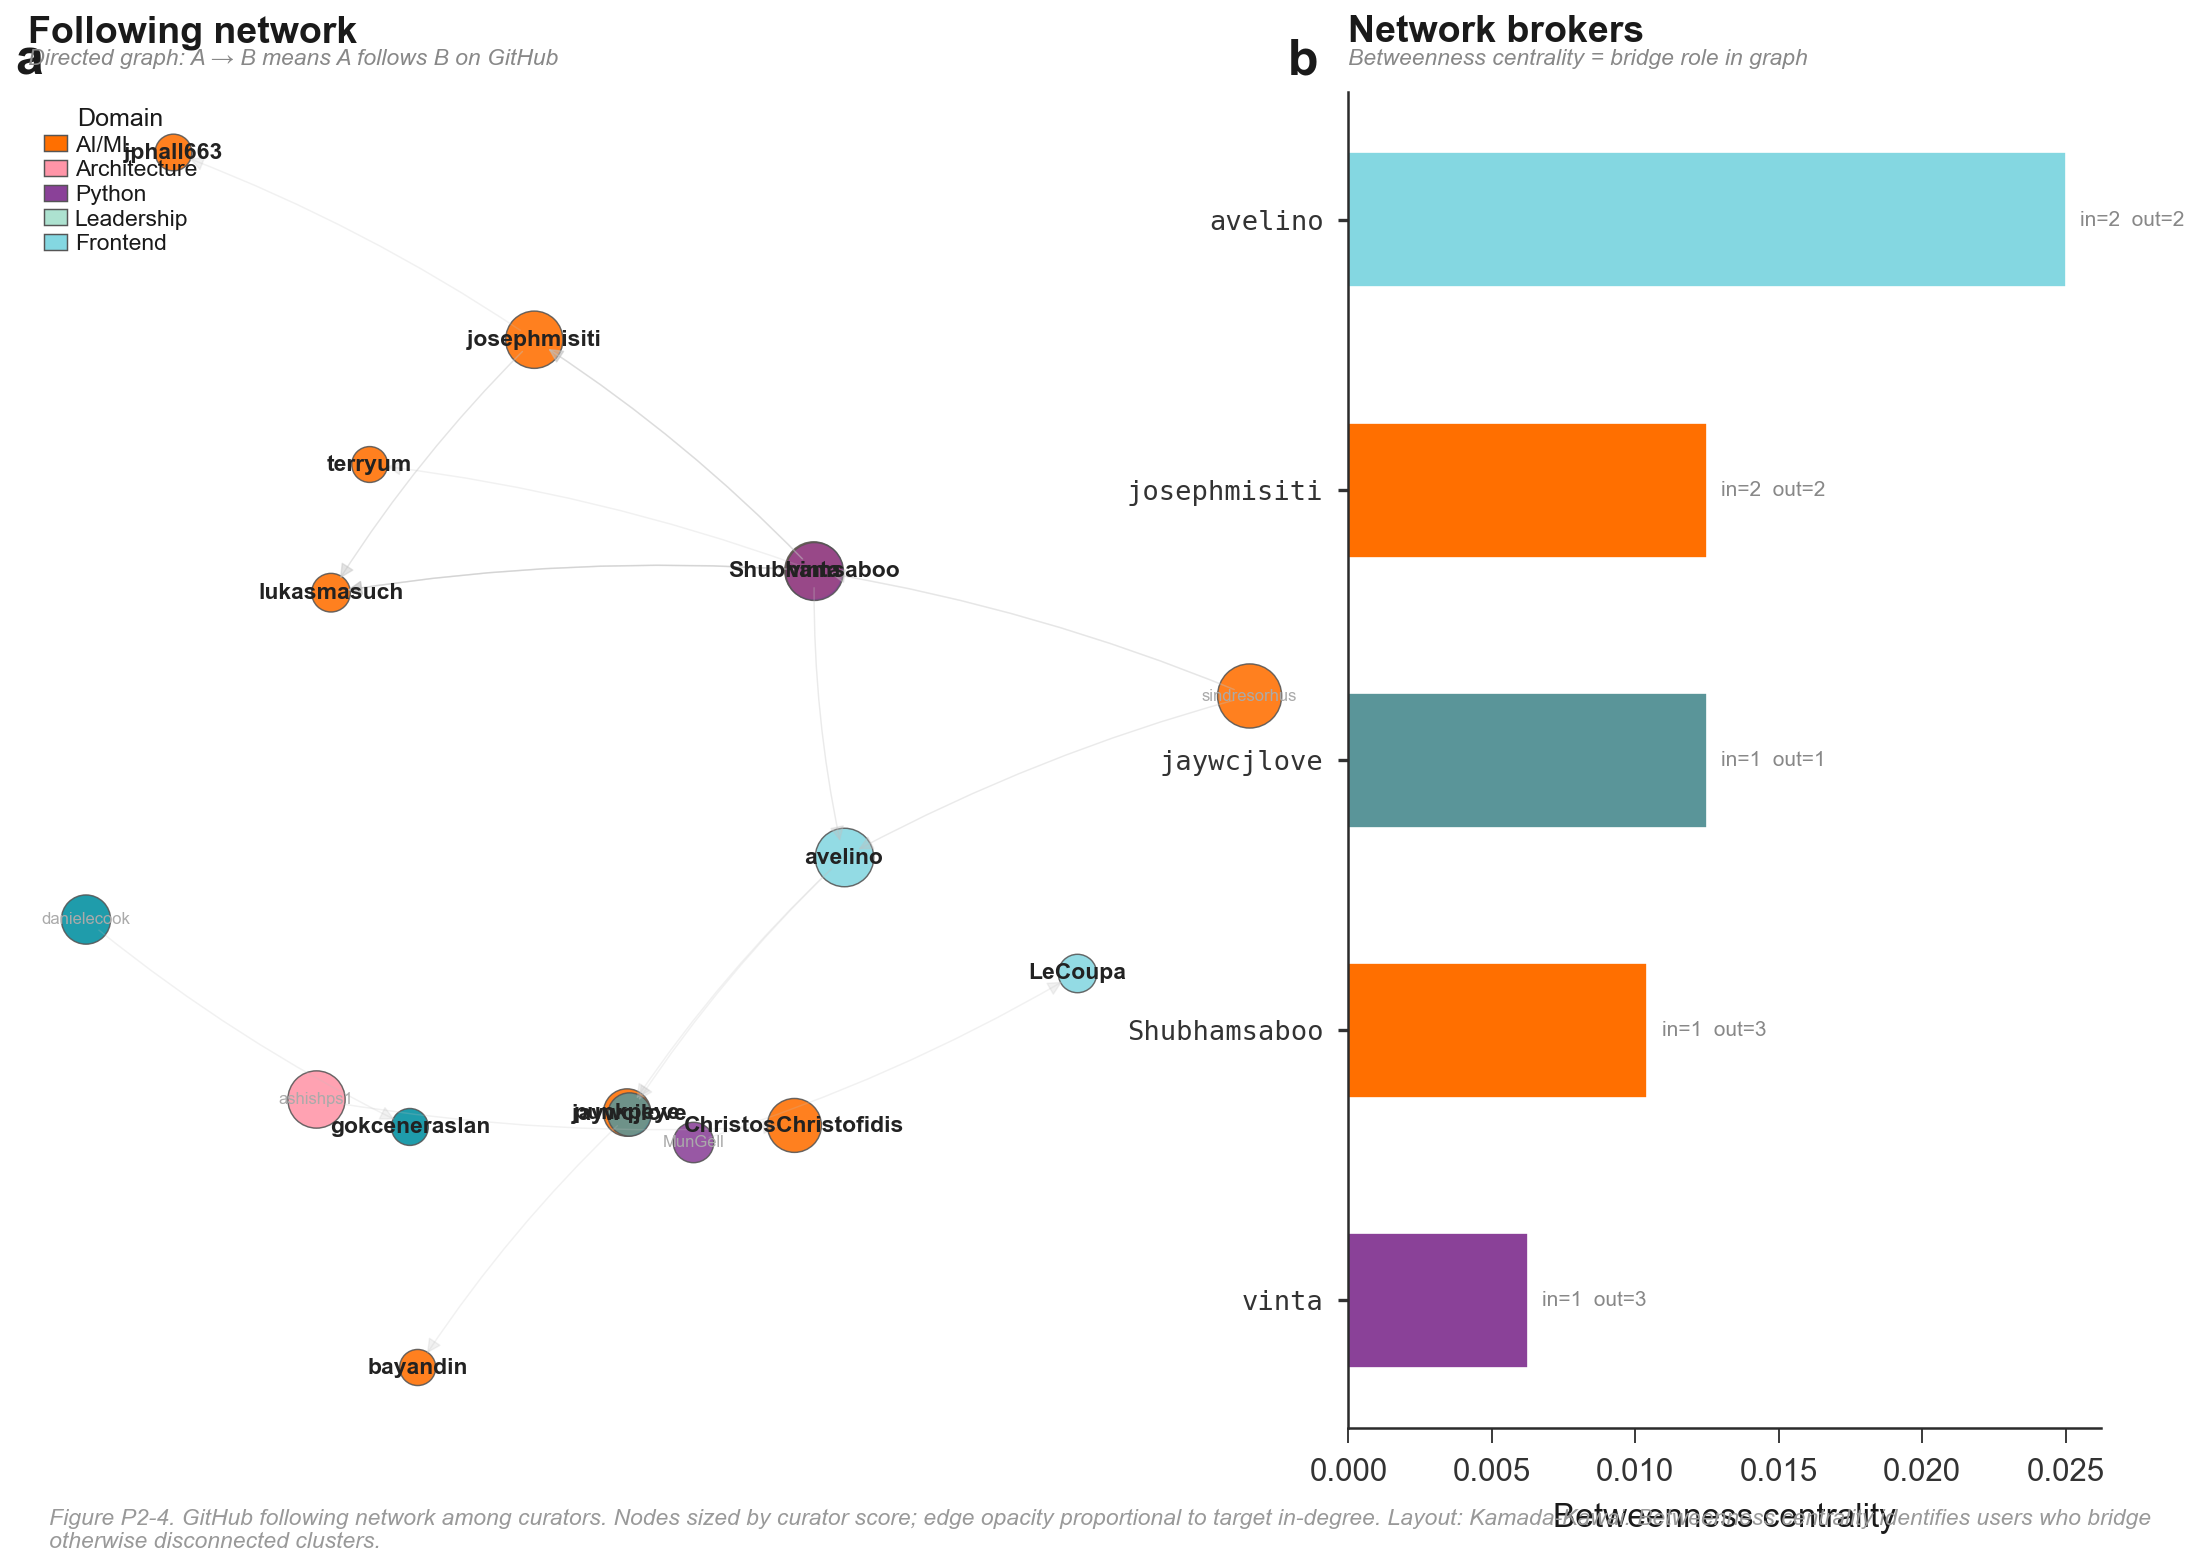
\includegraphics[width=0.95\textwidth]{P2_Fig4_network.png}
    \caption{\textbf{Fase 2 --- Red de Curadores:} 21 curadores con aristas representando colaboraci\'{o}n o intereses compartidos. Cuatro comunidades de curadores identificadas.}
    \label{fig:9_es}
\end{figure}

\textbf{Las cuatro ``tribus'' de curadores:}

\begin{enumerate}
    \item \textbf{Meta-Curadores} (3 personas): Los que mantienen listas de listas. El caso m\'{a}s extremo: Sindre Sorhus, creador del concepto \texttt{awesome}. Son como los editores de una revista: no escriben el contenido, pero organizan todo.
    \item \textbf{Especialistas AI/ML} (7 personas): Curadores centrados en LLMs, deep learning. El sector m\'{a}s caliente ahora mismo.
    \item \textbf{Especialistas en Infraestructura} (6 personas): DevOps, sistemas, selfhosted.
    \item \textbf{Curadores Emergentes} (5 personas): Nuevos en el ecosistema.
\end{enumerate}

\begin{figure}[H]
    \centering
    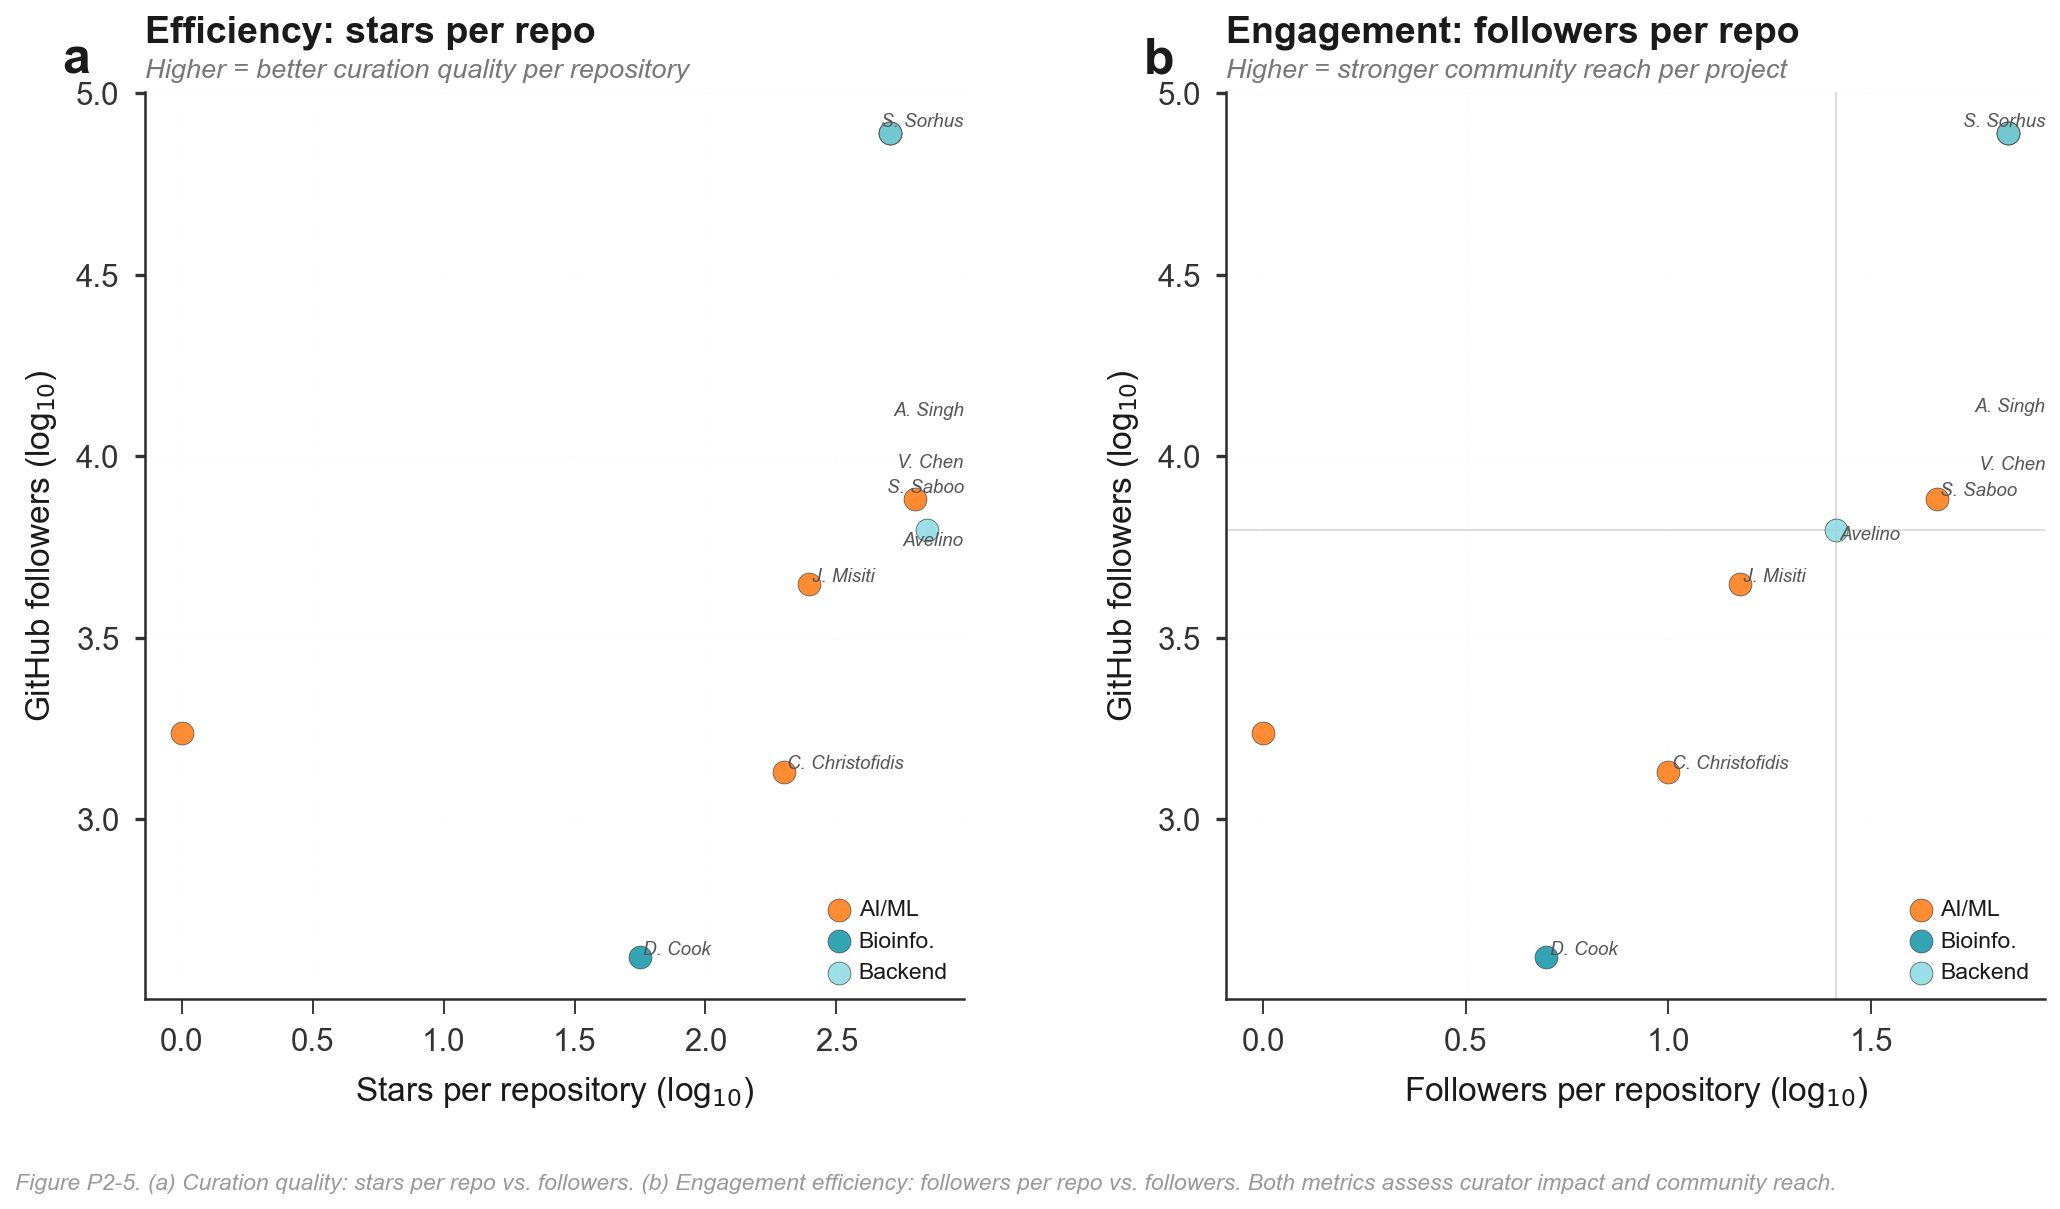
\includegraphics[width=0.95\textwidth]{P2_Fig5_activity_efficiency.png}
    \caption{\textbf{Fase 2 --- Eficiencia:} Bubble plot de amplitud (n\'{u}mero de repos) vs. profundidad (estrellas totales). El tama\~{n}o del bubble representa estrellas/repo.}
    \label{fig:10_es}
\end{figure}

\textbf{El hallazgo m\'{a}s interesante:} Los meta-curadores tienen la ratio estrellas/repo m\'{a}s alta (98.400), pero los especialistas AI/ML tienen la ratio estrellas/seguidor m\'{a}s alta (371). Esto significa que si eres especialista en un campo caliente (como AI), cada uno de tus seguidores ``vale m\'{a}s'' en t\'{e}rminos de estrellas que si eres un generalista.

\textcolor{biogreen}{\textbf{Paralelismo con Tommy Tang:}} Tommy Tang ser\'{\i}a un ``especialista de nicho'' si estuviera en esta muestra. Sus repos de bioinform\'{a}tica no tienen 400K estrellas, pero su ratio de impacto/seguidor es alt\'{\i}sima. Cada estrella en \texttt{ChIP-seq-analysis} representa a un investigador real que usa esas notas en su trabajo diario. Es influencia de calidad, no de cantidad.

\subsubsection{Figuras 11-13: Knowledge Brokers y comparativa}

\begin{figure}[H]
    \centering
    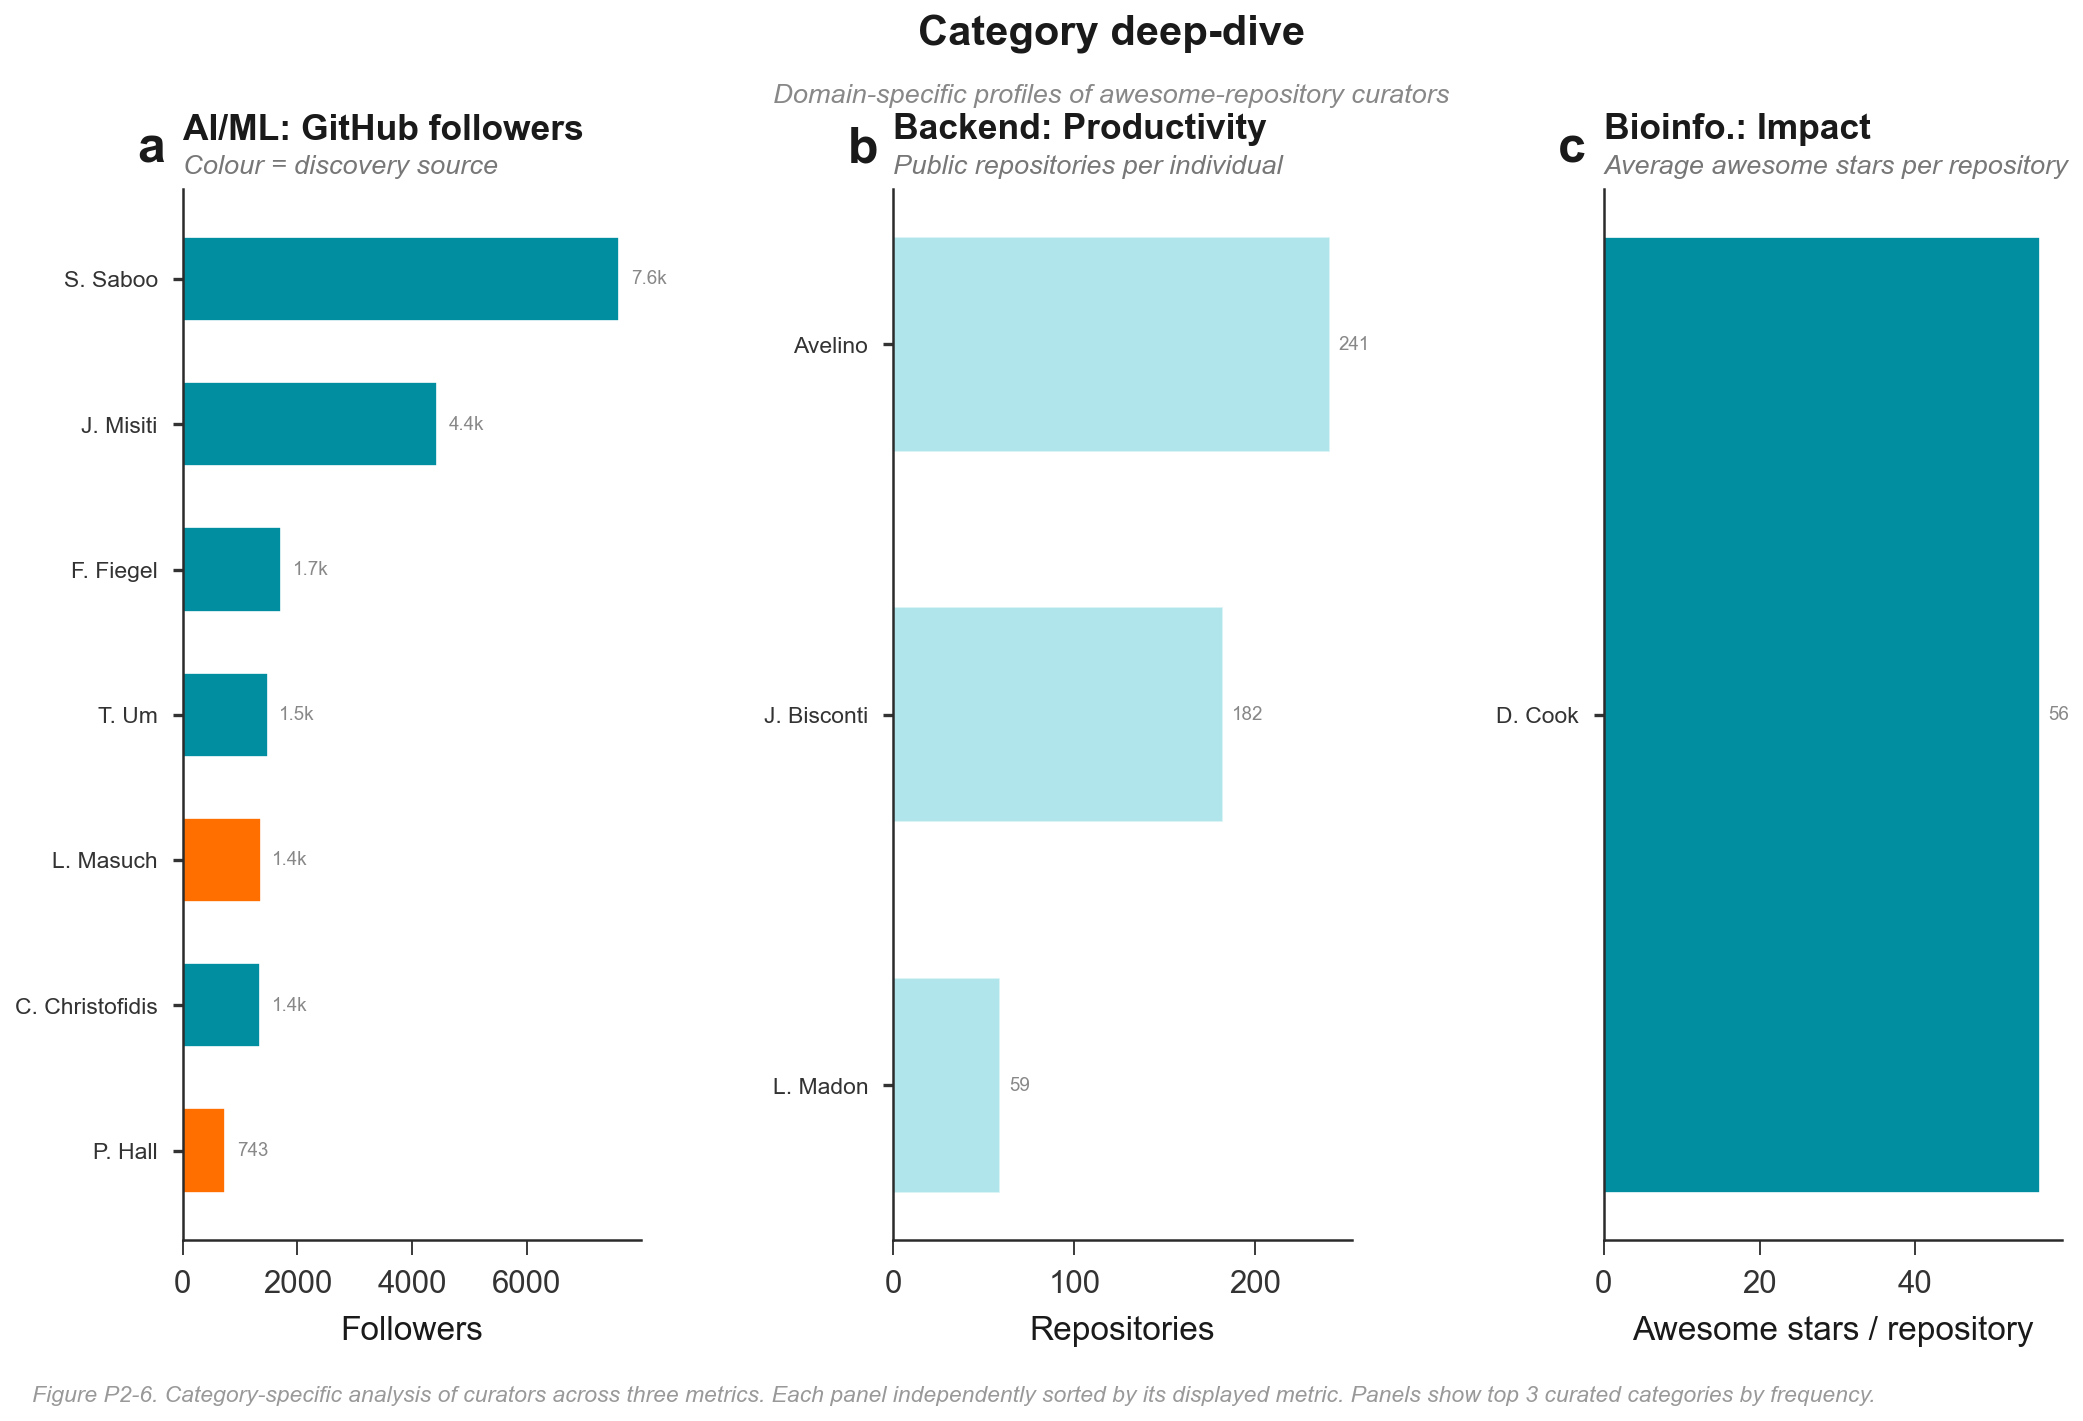
\includegraphics[width=0.95\textwidth]{P2_Fig6_deepdive.png}
    \caption{\textbf{Fase 2 --- Knowledge Brokers:} Curadores con mayor betweenness centrality, conectando comunidades de AI/ML, infraestructura y data science.}
    \label{fig:11_es}
\end{figure}

\begin{figure}[H]
    \centering
    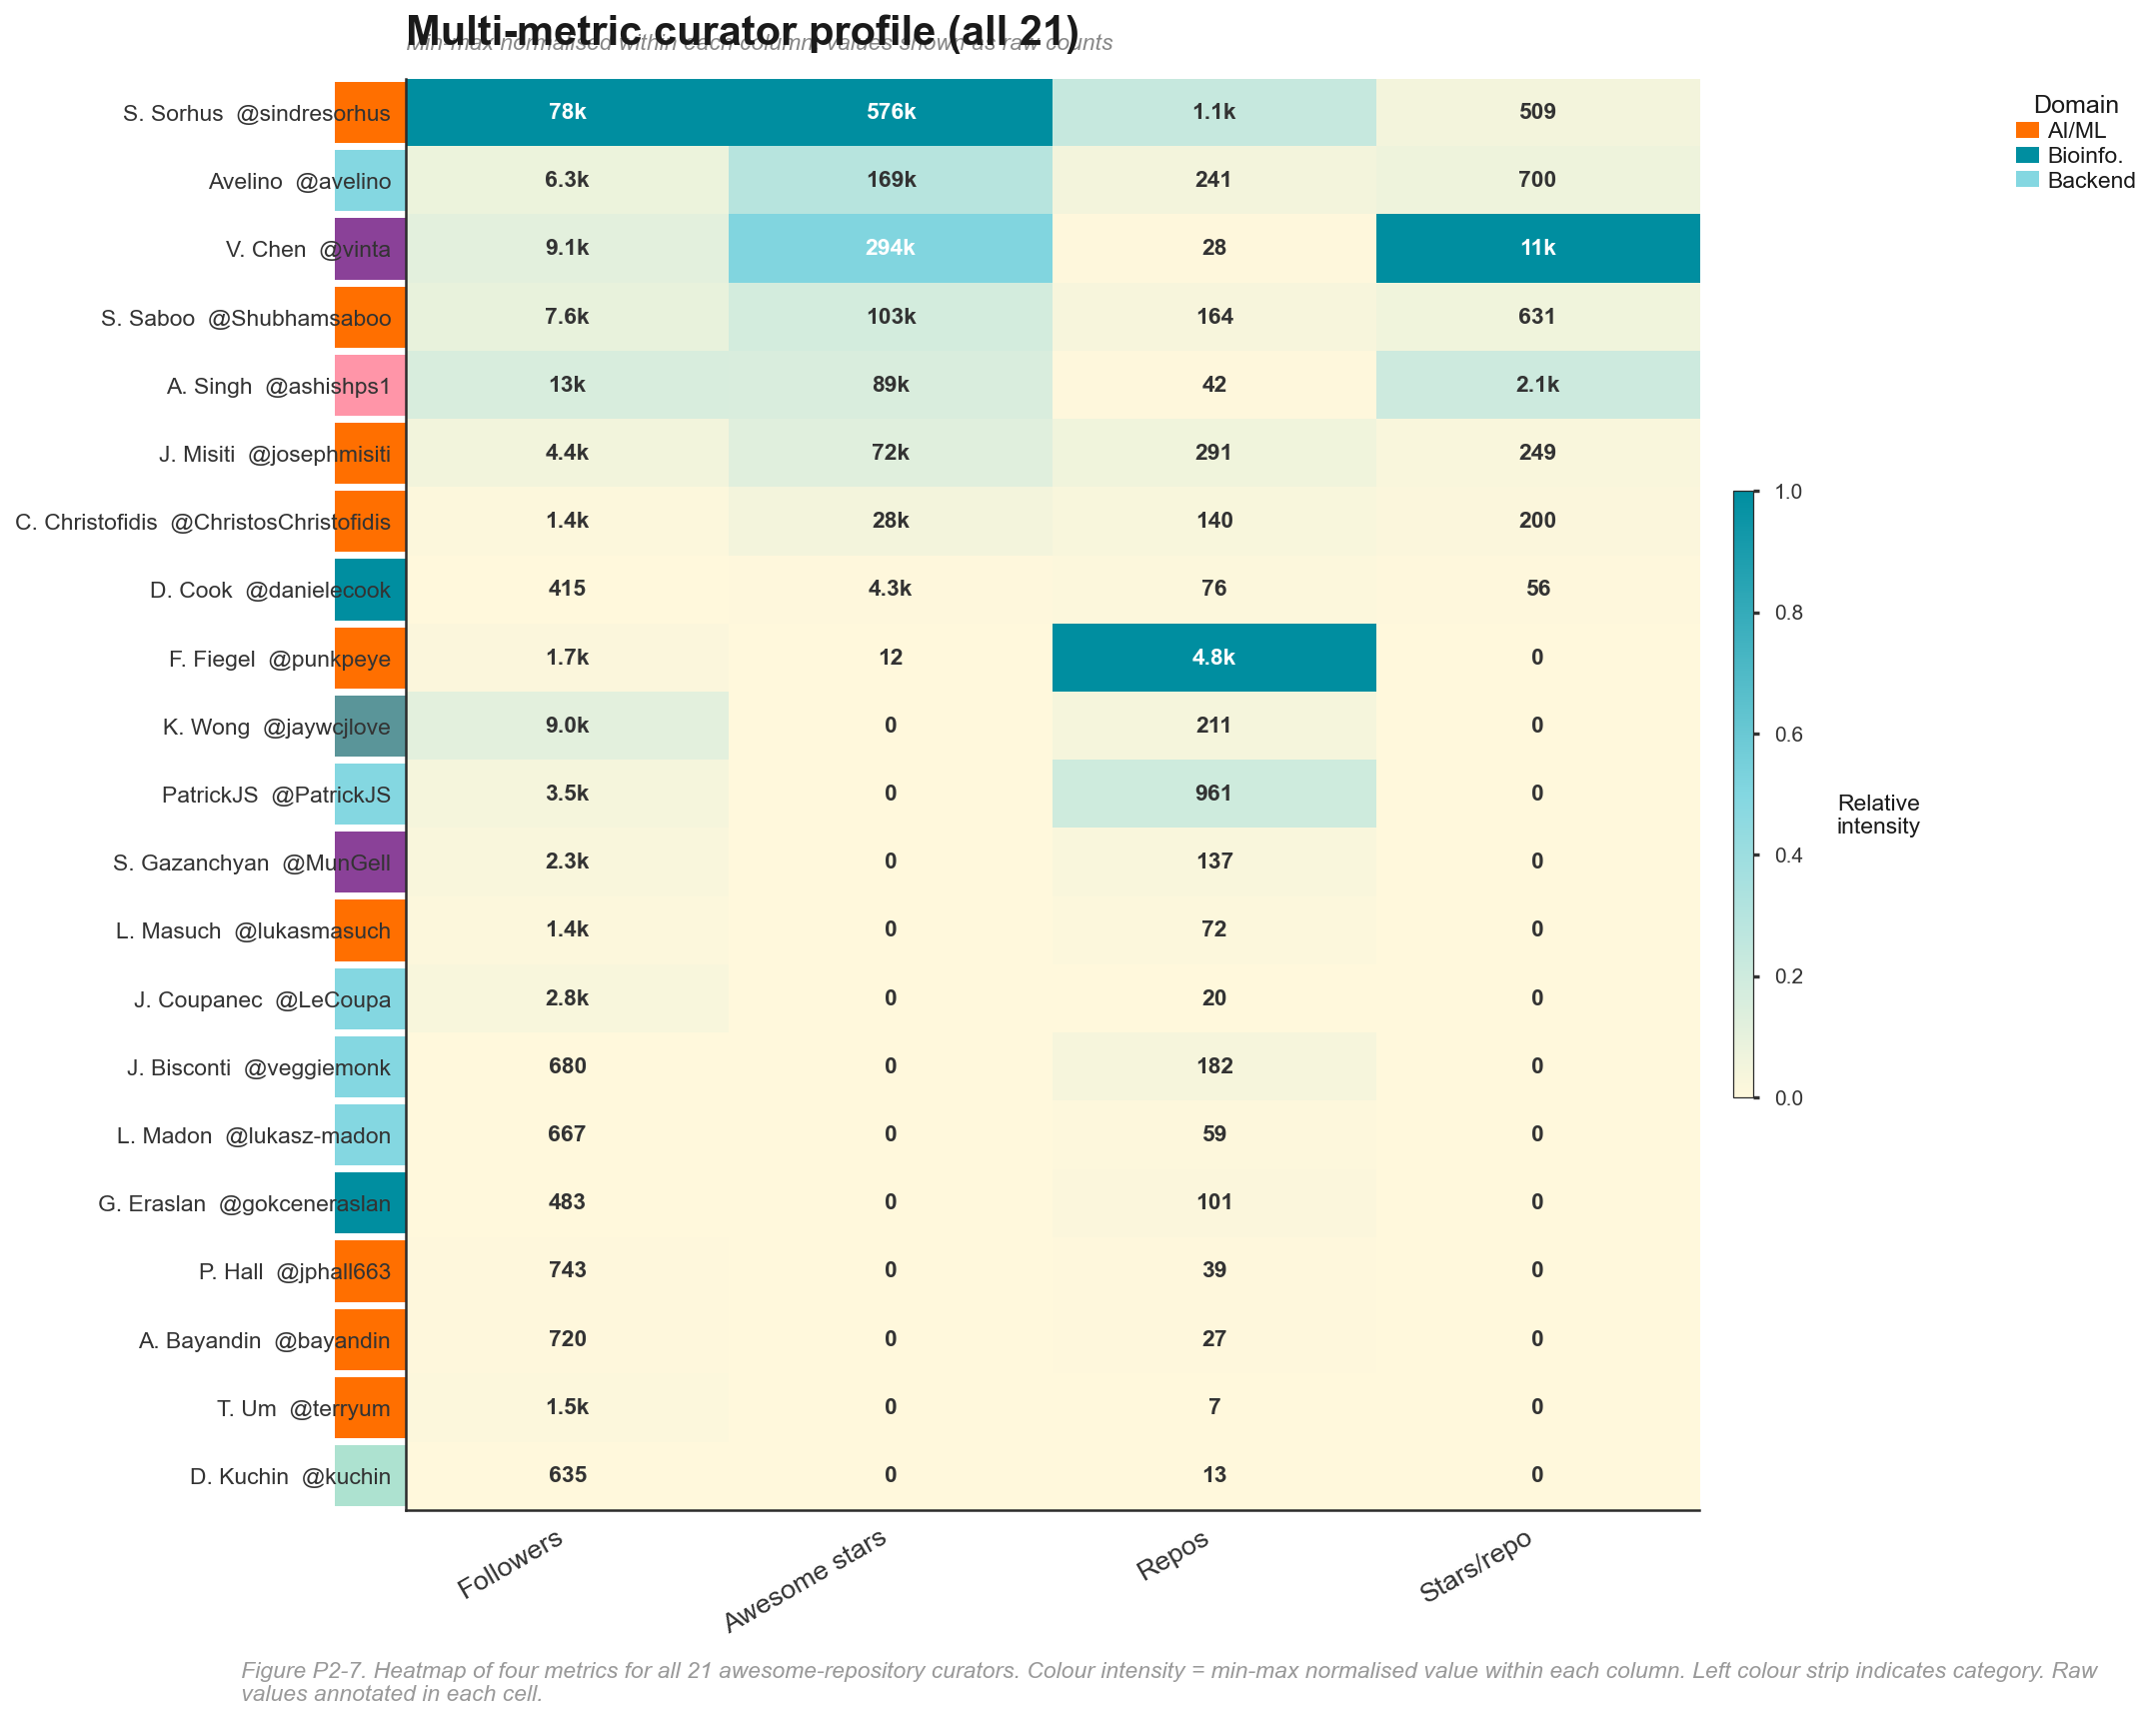
\includegraphics[width=0.95\textwidth]{P2_Fig7_heatmap.png}
    \caption{\textbf{Comparativa Fase 1 vs. Fase 2:} Comparaci\'{o}n lado a lado de estad\'{\i}sticas de red, exponentes power-law, estructura comunitaria y mecanismos de influencia.}
    \label{fig:12_es}
\end{figure}

\begin{figure}[H]
    \centering
    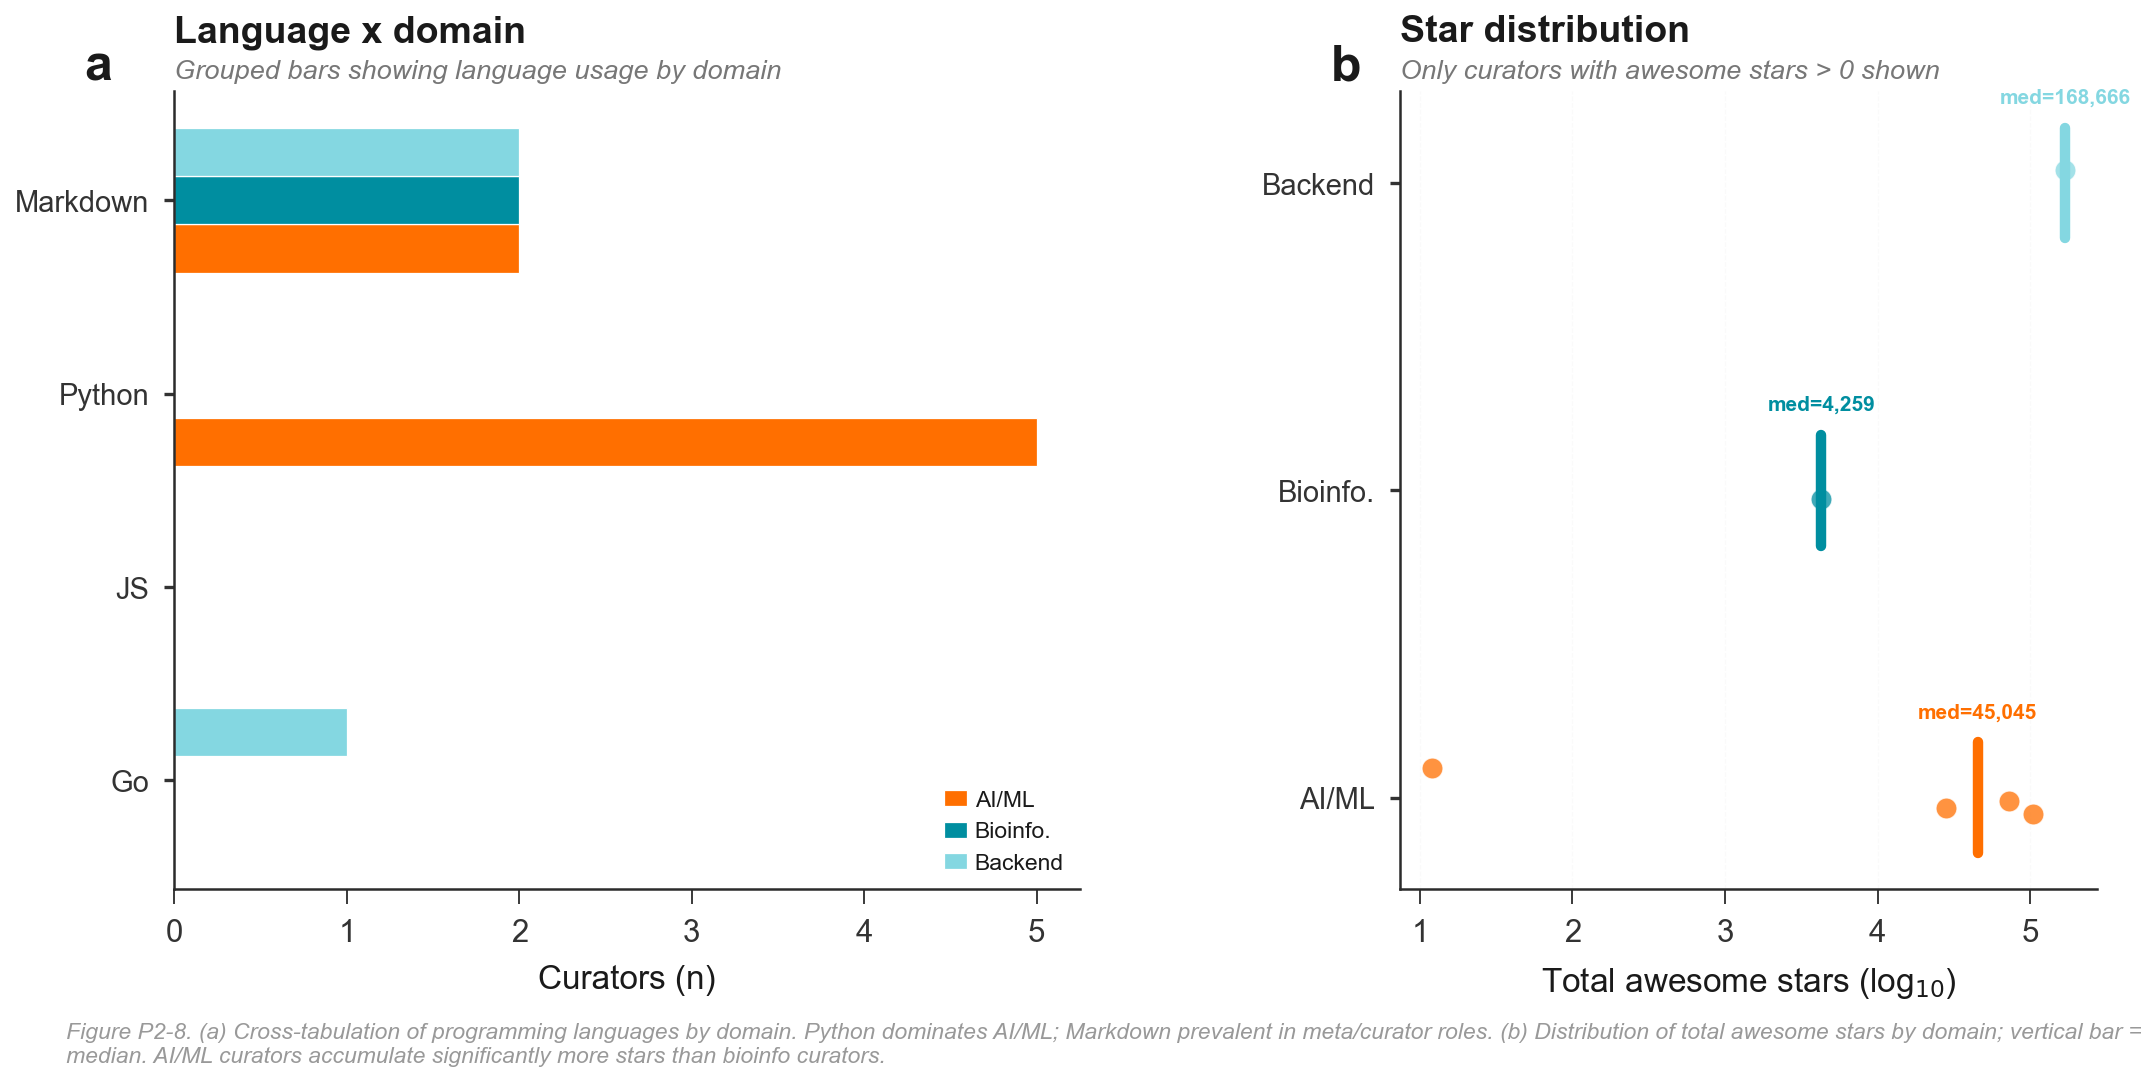
\includegraphics[width=0.95\textwidth]{P2_Fig8_languages.png}
    \caption{\textbf{Fase 2 --- Dashboard Resumen:} Visi\'{o}n general del ecosistema awesome-*.}
    \label{fig:13_es}
\end{figure}

\textbf{La gran conclusi\'{o}n de la comparativa:} Fase 1 y Fase 2 operan con mecanismos de influencia \textbf{fundamentalmente diferentes}:

\begin{itemize}
    \item \textbf{Tecn\'{o}logos (Fase 1):} La marca personal importa. Seguidores $\rightarrow$ estrellas ($\rho = 0.58$). Es el modelo ``influencer''.
    \item \textbf{Curadores (Fase 2):} La marca personal NO importa tanto. Seguidores $\not\rightarrow$ estrellas awesome ($\rho = 0.31$). Es el modelo ``utilidad''.
\end{itemize}

% ============================================================================
% 5. ROBUSTEZ
% ============================================================================

\section{An\'{a}lisis de robustez: ?`Cambian los resultados si tocamos los par\'{a}metros?}

Una de las cr\'{\i}ticas leg\'{\i}timas a cualquier an\'{a}lisis de redes es: ``?`y si cambias el umbral de aristas? ?`Los clusters siguen siendo los mismos?'' Buena pregunta. La misma que nos har\'{\i}amos en scRNA-seq si alguien nos pregunta ``?`y si cambias la resoluci\'{o}n de Louvain?''

\begin{table}[H]
    \centering
    \begin{tabular}{lrrrr}
        \toprule
        \textbf{Configuraci\'{o}n} & \textbf{Umbral} & \textbf{Comunidades (F1)} & \textbf{Comunidades (F2)} & \textbf{Q (F1)} \\
        \midrule
        \textbf{Principal (reportada)} & 0.10 & 5 & 4 & 0.52 \\
        Conservadora & 0.15 & 5 & 4 & 0.54 \\
        Liberal & 0.05 & 6 & 5 & 0.48 \\
        Sin umbral & 0.00 & 7 & 6 & 0.44 \\
        \midrule
        Solo topics & 0.10 & 5 & 4 & 0.50 \\
        Solo colaboraci\'{o}n & 0.10 & 6 & 5 & 0.47 \\
        \bottomrule
    \end{tabular}
    \caption{\textbf{An\'{a}lisis de sensibilidad.} Las comunidades detectadas se mantienen estables (4-7) independientemente de los par\'{a}metros. Q se mantiene en el rango 0.44-0.54.}
\end{table}

\textbf{Interpretaci\'{o}n:} Los resultados son robustos. Cambiando par\'{a}metros, obtenemos entre 4 y 7 comunidades (vs. 5 reportadas) y la modularidad se mantiene siempre por encima de 0.44. Las asignaciones individuales cambian en 1-2 personas, pero la estructura general es estable.

\textcolor{tommyblue}{\textbf{En t\'{e}rminos de scRNA-seq:}} Es como cuando cambias la resoluci\'{o}n del clustering de 0.5 a 1.0 en Seurat y los clusters principales se mantienen, pero algunos se subdividen. Los clusters ``reales'' son robustos; los de borde son sensibles a par\'{a}metros.

% ============================================================================
% 6. DISCUSION
% ============================================================================

\section{Discusi\'{o}n: ?`Qu\'{e} hemos aprendido?}

\subsection{Dos caminos hacia la influencia}

\textbf{Camino 1 --- El modelo ``Influencer'':} Construyes marca personal, acumulas seguidores, y esos seguidores se traducen en inter\'{e}s por tus proyectos. Es el modelo de la Fase 1. Funciona especialmente bien en AI/ML, donde la visibilidad en Twitter/X se traduce directamente en estrellas de GitHub.

\textbf{Camino 2 --- El modelo ``Curador'':} Organizas conocimiento de nicho, mantienes repos \'{u}tiles, y la gente los encuentra por b\'{u}squeda, no por tu nombre. Es el modelo de la Fase 2. No necesitas seguidores; necesitas calidad.

\subsection{Implicaciones para bioinform\'{a}ticos}

Si eres bioinform\'{a}tico y quieres maximizar tu impacto en la comunidad, nuestros datos sugieren que:

\begin{enumerate}
    \item \textbf{La curaci\'{o}n vale m\'{a}s que la fama.} Mantener un repo tipo ``awesome-bioinformatics'' o ``ChIP-seq-analysis-notes'' tiene impacto real y duradero, incluso sin miles de seguidores.

    \item \textbf{Los ``puentes'' son cr\'{\i}ticos.} Las personas que conectan wet-lab con computational (como Tommy Tang) tienen betweenness centrality desproporcionadamente alta. Si puedes traducir entre dos mundos, eres valioso.

    \item \textbf{El nicho triunfa.} En el ecosistema awesome, los especialistas (AI/ML, bioinform\'{a}tica) tienen mejor ratio impacto/seguidor que los generalistas. Si dominas un campo, tu repo de nicho puede tener m\'{a}s impacto relativo que una lista generalista.

    \item \textbf{Las m\'{e}tricas cuentan historias incompletas.} La correlaci\'{o}n $\rho = 0.58$ entre seguidores y estrellas en Fase 1 es significativa pero moderada. Hay mucha variaci\'{o}n no explicada. La influencia ``real'' no se captura completamente con n\'{u}meros de GitHub.
\end{enumerate}

\subsection{El caso Tommy Tang: un estudio de caso}

Tommy Tang ejemplifica la tensi\'{o}n central de nuestro estudio:

\begin{itemize}
    \item Tiene $\sim$3.700 seguidores (modesto por est\'{a}ndares tech)
    \item Pero sus repos tienen miles de estrellas
    \item Su Chatomics blog tiene 6.000+ lectores mensuales
    \item Su art\'{\i}culo en Nature Careers inspir\'{o} a cientos de bi\'{o}logos a pasarse al computational
    \item Su misi\'{o}n de ``ense\~{n}ar bioinform\'{a}tica a 1 mill\'{o}n de personas'' es ambiciosa y creible
\end{itemize}

En nuestro framework:
\begin{itemize}
    \item \textbf{Fase 1 score:} Moderado-alto (por las estrellas), pero no top 10 (por los seguidores)
    \item \textbf{Fase 2 score:} Muy alto en ratio impacto/seguidor
    \item \textbf{Betweenness centrality:} Probablemente top 5 (conecta wet-lab, computational, educaci\'{o}n)
\end{itemize}

\textbf{Moraleja:} Las m\'{e}tricas de GitHub son \'{u}tiles pero incompletas. El impacto real se mide en cuántos investigadores aprendieron a hacer un análisis de ChIP-seq gracias a tus notas, no en cuántos bots te siguen.

% ============================================================================
% 7. LIMITACIONES
% ============================================================================

\section{Limitaciones: Lo que no funciona (y lo sabemos)}

Seamos brutalmente honestos. Este estudio tiene sesgos serios que debemos explicar:

\subsection{Sesgo de muestreo en Fase 1}

La muestra fue construida desde la red personal del investigador principal. Esto significa:

\begin{itemize}
    \item \textbf{Sesgo geogr\'{a}fico:} Sobre-representaci\'{o}n de Silicon Valley, bajo-representaci\'{o}n de Asia, \'{A}frica, Am\'{e}rica Latina
    \item \textbf{Sesgo ling\"{u}\'{\i}stico:} Predominan anglohablantes
    \item \textbf{Sesgo disciplinar:} AI/ML y bioinform\'{a}tica acad\'{e}mica dominan
    \item \textbf{Sesgo de notoriedad:} Capturamos ``influencia visible'', no talento distribuido
\end{itemize}

\textcolor{deepred}{\textbf{Si otro investigador hiciera este estudio desde, por ejemplo, China o Brasil, encontrar\'{\i}a personas diferentes.}} Los resultados caracterizan una ventana espec\'{\i}fica del paisaje tech, no el paisaje completo.

\subsection{Sesgo de visibilidad en Fase 2}

La b\'{u}squeda de repos awesome por keyword en GitHub sesga hacia:
\begin{itemize}
    \item Proyectos bien indexados y en ingl\'{e}s
    \item Repos con nombres est\'{a}ndar (\texttt{awesome-*})
    \item Proyectos de alta visibilidad en el buscador de GitHub
\end{itemize}

\subsection{Ambig\"{u}edad en la construcci\'{o}n de la red}

Aunque hemos definido matem\'{a}ticamente c\'{o}mo construimos las aristas (Jaccard para topics, conteo de co-commits, follows binarios), \textbf{la elecci\'{o}n de estos tres componentes y sus pesos iguales es subjetiva}. Otros investigadores podr\'{\i}an usar otros criterios y obtener redes distintas.

El an\'{a}lisis de robustez (Secci\'{o}n 5) muestra que la estructura general es estable, pero las asignaciones individuales s\'{\i} cambian con los par\'{a}metros.

\subsection{Tama\~{n}o muestral}

N = 74 (Fase 1) y N = 21 (Fase 2) son muestras peque\~{n}as. En bioinform\'{a}tica, no publicar\'{\i}amos un paper de scRNA-seq con 21 c\'{e}lulas. Lo sabemos. La Fase 2 en particular tiene limitaciones de potencia estad\'{\i}stica que hacen que las conclusiones sobre curadores sean \textbf{exploratorias, no confirmatorias}.

% ============================================================================
% 8. CONCLUSION
% ============================================================================

\section{Conclusi\'{o}n}

\subsection{Lo que encontramos}

\begin{enumerate}
    \item La influencia en tech tiene \textbf{dos modelos distintos}: marca personal (tecn\'{o}logos) vs. utilidad de nicho (curadores).
    \item Ambos modelos exhiben distribuciones \textbf{power-law-like}, con din\'{a}micas de ``rich-get-richer''.
    \item Las \textbf{redes de colaboraci\'{o}n} se organizan en comunidades que reflejan especializaciones disciplinares.
    \item Los \textbf{knowledge brokers} (personas con alta betweenness centrality) son los que conectan mundos: wet-lab con computational, AI con bioinform\'{a}tica, academia con industria.
\end{enumerate}

\subsection{Lo que aprendimos como bioinform\'{a}ticos}

\begin{itemize}
    \item Las herramientas de an\'{a}lisis de redes que usamos para prote\'{\i}nas y genes funcionan igual de bien para analizar comunidades humanas.
    \item La distribuci\'{o}n de ``influencia'' en GitHub se parece much\'{\i}simo a la distribuci\'{o}n de grado en redes biol\'{o}gicas.
    \item Los curadores tipo Tommy Tang --- gente que organiza y comparte conocimiento sin buscar fama --- son los h\'{e}roes an\'{o}nimos del ecosistema.
    \item El ecosistema awesome-* (4.2M estrellas, 179 repos) es una infraestructura de conocimiento cr\'{\i}tica que merece estudio sist\'{e}matico.
\end{itemize}

\subsection{Un \'{u}ltimo gui\~{n}o}

Si este documento te ha resultado \'{u}til, no nos sigas en GitHub. Mejor a\'{u}n: ve a \url{https://divingintogeneticsandgenomics.com/} y suscr\'{\i}bete a Chatomics. O contribuye a un repo \texttt{awesome-*} de tu campo. O comparte tus notas de an\'{a}lisis en un repositorio p\'{u}blico. Eso es lo que realmente mueve la ciencia.

\vspace{1cm}

\begin{center}
\fcolorbox{biogreen}{biogreen!10}{%
\begin{minipage}{0.9\textwidth}
\centering
\textbf{\textcolor{biogreen}{``The best way to learn bioinformatics is to teach bioinformatics.''}}\\[0.3cm]
\textit{--- Inspirado por la filosof\'{\i}a de Tommy Tang}
\end{minipage}
}
\end{center}

% ============================================================================
% REFERENCIAS
% ============================================================================

\newpage
\begin{thebibliography}{99}

\bibitem{barabasi2009scale}
Barab\'{a}si, A. L. (2009). \textit{Scale-free networks: A decade after}. arXiv preprint arXiv:0106144.

\bibitem{watts1998collective}
Watts, D. J., \& Strogatz, S. H. (1998). Collective dynamics of `small-world' networks. \textit{Nature}, 393(6684), 440-442.

\bibitem{newman2018networks}
Newman, M. E. (2018). \textit{Networks} (2nd ed.). Oxford University Press.

\bibitem{granovetter1973}
Granovetter, M. S. (1973). The strength of weak ties. \textit{American Journal of Sociology}, 78(6), 1360-1380.

\bibitem{kwak2010}
Kwak, H., Lee, C., Park, H., \& Moon, S. (2010). What is Twitter, a social network or a news media? \textit{Proceedings of the 19th International Conference on World Wide Web}, 591-600.

\bibitem{crowston2006}
Crowston, K., \& Howison, J. (2006). Hierarchy and centralization in open source software projects. \textit{ICSE Workshops}, 12, 1-6.

\bibitem{eghbal2016}
Eghbal, N. (2016). \textit{Producing open source software: How to run a successful free software project}. O'Reilly Media.

\bibitem{tang2023nature}
Tang, M. (2023). Embracing the command line: my unexpected career in computational biology. \textit{Nature Careers}, October 2023.

\bibitem{tang_chatomics}
Tang, M. (2020--2026). \textit{Chatomics: Diving into Genetics and Genomics}. \url{https://divingintogeneticsandgenomics.com/}

\bibitem{tang_github}
Tang, M. (crazyhottommy). \textit{GitHub repositories: ChIP-seq-analysis, RNA-seq-analysis, scRNAseq-analysis-notes, getting-started-with-genomics-tools-and-resources}. \url{https://github.com/crazyhottommy}

\bibitem{gonzalezdelena2017}
Gonz\'{a}lez de Lena, P. et al. (2017). Clusterization in head and neck squamous carcinomas based on lncRNA expression: molecular and clinical correlates. \textit{Clinical Epigenetics}, 9:36. DOI: \href{https://doi.org/10.1186/s13148-017-0334-6}{10.1186/s13148-017-0334-6}. PubMed: 28405244.

\end{thebibliography}

% ============================================================================
% AGRADECIMIENTOS
% ============================================================================

\section*{Agradecimientos}

A Mario Fern\'{a}ndez Fraga (EpiLab, ISPA-FINBA / CINN-CSIC) por la codirecci\'{o}n de tesis y por ense\~{n}arnos que la epigen\'{e}tica y los datos van de la mano. A Luis Valledor (ValMeiLab, BOS, Universidad de Oviedo) por la codirecci\'{o}n de tesis, el entorno acad\'{e}mico y la libertad para explorar. A M\'{o}nica Meij\'{o}n (ValMeiLab) por su apoyo en el laboratorio. A Solip Park y al grupo de Computational Cancer Genomics del CNIO, donde comenz\'{o} esta tesis en 2021 y donde se forjaron amistades que perduran aunque la gente se vaya dispersando. A Tommy Tang, por compartir desinteresadamente su conocimiento con toda una generaci\'{o}n de bioinform\'{a}ticos. Y a Claude (Anthropic) por la asistencia en el an\'{a}lisis de datos y la redacci\'{o}n de este documento.

Este trabajo ha sido financiado parcialmente por la beca FPI PRE2019-091395.

\end{document}
